%\documentclass[a4paper]{article}
%\usepackage{geometry}
%\geometry{a4paper,scale=0.8}
\documentclass[8pt]{article}
\usepackage{ctex}
\usepackage{indentfirst}
\usepackage{longtable}
\usepackage{multirow}
\usepackage[a4paper, total={6.5in, 9in}]{geometry}
\usepackage{CJK}
\usepackage[fleqn]{amsmath}
\usepackage{parskip}
\usepackage{listings}
\usepackage{fancyhdr}

\pagestyle{fancy}

% 设置页眉
\fancyhead[L]{2024年秋季}
\fancyhead[C]{机器学习}
\fancyhead[R]{作业四}


\usepackage{graphicx}
\usepackage{float}
\usepackage{multicol}
\usepackage{amssymb}
\usepackage{booktabs}
\usepackage{xcolor}

% 定义Python代码风格
\definecolor{codegreen}{rgb}{0,0.6,0}
\definecolor{codegray}{rgb}{0.5,0.5,0.5}
\definecolor{codepurple}{rgb}{0.58,0,0.82}
\definecolor{backcolour}{rgb}{0.95,0.95,0.92}

\lstdefinestyle{mystyle}{
    backgroundcolor=\color{backcolour},   
    commentstyle=\color{codegreen},
    keywordstyle=\color{magenta},
    numberstyle=\tiny\color{codegray},
    stringstyle=\color{codepurple},
    basicstyle=\ttfamily\footnotesize,
    breakatwhitespace=false,         
    breaklines=true,     
    captionpos=b,        
    keepspaces=true,     
    numbers=left,        
    numbersep=5pt,       
    showspaces=false,    showstringspaces=false,
    showtabs=false,      
    tabsize=2
}

\lstset{style=mystyle}
\begin{document}

\textbf{\color{blue} \Large 姓名:毛九弢 \ \ \ 学号:221900175 \ \ \ \today}


\section*{一. (30 points) 随机森林的原理}

集成学习是一种通用技术,通过将多个不同模型的预测结果结合起来,以平均值或多数投票的方式生成单一预测,从而有效应对过拟合问题。


1. 考虑一组互不相关的随机变量 $\{Y_i\}_{i=1}^n$,其均值为 $\mu$,方差为 $\sigma^2$。  
请计算这些随机变量平均值的期望和方差,给出计算过程。  
提示:在集成方法的背景下,这些 $Y_i$ 类似于分类器 $i$ 所作的预测。(5 points)

\textbf{\large 解:}

设 $Y_i$ 的平均值为 $\bar{Y} = \frac{1}{n} \sum_{i=1}^n Y_i$。

(1) 期望:根据期望线性性质,有:
\[
E(\bar{Y}) = E\left(\frac{1}{n} \sum_{i=1}^n Y_i\right) = \frac{1}{n} \sum_{i=1}^n E(Y_i) = \frac{1}{n} \sum_{i=1}^n \mu = \mu
\]

(2) 方差:

由于 $Y_i$ 互不相关,各协方差为0,即,和的方差等于各自方差之和。

所以有:
\[
\operatorname{Var}(\bar{Y}) = \operatorname{Var}\left(\frac{1}{n} \sum_{i=1}^n Y_i\right) = \frac{1}{n^2} \sum_{i=1}^n \operatorname{Var}(Y_i) = \frac{1}{n^2} \sum_{i=1}^n \sigma^2 = \frac{\sigma^2}{n}
\]

因此,这些随机变量平均值的期望为 $\mu$,方差为 $\frac{\sigma^2}{n}$。

\vspace{3em}

2. 在第1小问中,我们看到对于不相关的分类器,取平均可以有效减少方差。  
尽管现实中的预测不可能完全不相关,但降低决策树之间的相关性通常能减少最终方差。  
现在,重新考虑一组具有相关性的随机变量 $\{Z_i\}_{i=1}^n$,其均值为 $\mu$,方差为 $\sigma^2$,每个 $Z_i \in \mathbb{R}$ 为标量。  
假设对任意 $i \neq j$,$\operatorname{Corr}(Z_i, Z_j) = \rho$。  
提示:如果你不记得相关性与协方差之间的关系,请回顾你的概率论等课程内容。 
\begin{itemize}
\item
请计算随机变量 $Z_i$ 平均值的方差,以 $\sigma$、$\rho$ 和 $n$ 为变量表示,给出计算过程。(5 points)  
\item
当 $n$ 非常大时,会发生什么?这对于取平均的潜在有效性说明了什么?  
(……如果 $\rho$ 很大($| \rho | \approx 1$)会怎样?……如果 $\rho$ 非常小($|\rho| \approx 0$)又会怎样?……如果 $\rho$ 处于中等水平($|\rho| \approx 0.5$)呢?)  
无需严格推导——基于你得出的方差公式,用定性分析进行讨论即可。 (6 points)
\end{itemize}

\textbf{\large 解:}
\[
    \operatorname{Var}\left(\sum_{i=1}^{n}X_i\right)
=
\sum_{i=1}^{n}\operatorname{Var}\left(X_i\right)
+
2\sum_{i=1}^{n-1}\sum_{j=i+1}^{n}\operatorname{Cov}\left(X_i,X_j\right)
\]

(1) 随机变量 $Z_i$ 平均值的方差
\begin{align*}
& \operatorname{Var}(\bar{Z}) 
= \operatorname{Var}\left(\frac{1}{n} \sum_{i=1}^n Z_i\right) 
\\ & = \frac{1}{n^2} 
    \left(
    \sum_{i=1}^n \operatorname{Var}(Z_i)
    +
    2 \sum_{i=1}^{n-1} \sum_{j=i+1}^n \operatorname{Cov}(Z_i, Z_j)
    \right) 
= \frac{1}{n^2} 
    \left(
        \sum_{i=1}^n \operatorname{Var}(Z_i)
        +
        2 \sum_{i=1}^{n-1} \sum_{j=i+1}^n \operatorname{Corr}(Z_i, Z_j)\sigma^2
    \right) 
\\ &= \frac{1}{n^2} 
    \left(
        \sum_{i=1}^n \sigma^2 
        +
        2 \sum_{i=1}^{n-1} \sum_{j=i+1}^n \rho\sigma^2 
    \right)
= \frac{1 + (n-1)\rho}{n}\sigma^2
\end{align*}

(2)  当 $n$ 非常大时,这些随机变量$Z_i$平均值的方差会趋于 $\rho\sigma^2$。

(2.1) 如果 $\rho$ 很大($| \rho | \approx 1$), 那么方差会趋于 $\sigma^2$,即据平均值后,方差的期望与原先相比没有减小,说明取平均的有效性不明显。

(2.2) 如果 $\rho$ 非常小($|\rho| \approx 0$), 那么方差会趋于 $\sigma^2/n$,当 $n$ 非常大时,这个数趋于0,即据平均值后,方差的期望会大大减小,说明取平均的有效性明显。
    
(2.3) 如果 $\rho$ 处于中等水平($|\rho| \approx 0.5$)呢, 那么当 $n$ 非常大时,方差会趋于 $\frac{1}{2}\sigma^2$,即据平均值后,方差的期望会减小,说明取平均的有一定有效性。

但不管 $\rho$ 多大,取平均后的方差期望都不会比原先来得大,因此,概率上来看,取平均的有效性是有的,且$\rho$越小,取平均的有效性越好。

\vspace{3em}

3. Bagging 是一种通过随机化从同一数据集生成多个不同学习器的方法。给定一个大小为 $n$ 的训练集,Bagging 会通过有放回抽样生成 $T$ 个随机子样本集,每个子样本集大小为 $n'$。
在每个子样本集中,一些数据点可能会被多次选中,而另一些可能完全未被选中。
当 $n' = n$ 时,大约 $63\%$ 的数据点会被选中,而剩下的 $37\%$ 被称为袋外样本点(Out-of-Bag,OOB)。
\begin{itemize}
\item
为什么是 $63\%$?
提示:当 $n$ 很大时,某个样本点未被选中的概率是多少?请只考虑在任意一个子样本集中(而不是所有 $T$ 个子样本集)未被选中的概率。(7 points)
\item
关于决策树的数量 $T$。
集成中的决策树数量通常需要在运行时间和降低方差之间进行权衡(典型值范围从几十到几千棵树)。
而子样本大小 $n'$ 对运行时间的影响较小,因此选择 $n'$ 时主要考虑如何获得最优预测结果。
虽然常见实践是设置 $n' = n$,但这并非总是最佳选择。
你会如何建议我们选择超参数 $n'$? (7 points)
\end{itemize}

\textbf{\large 解:}

(1) 为什么是 $63\%$?

在$n'$次采样中,由于$n' = n$,所以一个样本从未被选中的概率是 $(1 - \frac{1}{n})^{n'} = (1 - \frac{1}{n})^{n}$,当 $n$ 很大时,这个概率趋于 $e^{-1} \approx 0.37$。
因此,在$n'$次采样中,一个样本被选中的概率趋于 $1 - 0.37 = 0.63$。

引入$I(x_i)$,表示在$n'$次采样中样本 $x_i$ 被选中的指示函数,那么 $E(I(x_i)) = 0.63$。
那么,被选中的不同的样本数的期望为$
E\left(\sum_{i=1}^{n}I(x_i)\right) 
= \sum_{i=1}^{n}E(I(x_i)) = 0.63n$。

那么,被选中的样本数占总样本数的比例为 $0.63$,即$63\%$。

(2) 关于决策树的数量 $T$ (超参数$n'$的选择)。

1. 数据集的大小:如果数据集较大,可以选择较大的 $n'$,以确保每个子样本集包含足够的信息。如果数据集较小,可以选择较小的 $n'$,以增加子样本集的多样性。

2. 模型的复杂度:如果模型较复杂,可以选择较大的 $n'$,以确保每个子样本集包含足够的信息。如果模型较简单,可以选择较小的 $n'$,以增加子样本集的多样性。

3. 交叉验证:可以通过交叉验证来选择最优的 $n'$,以确保模型的泛化能力。

总之,选择 $n'$ 时需要综合考虑数据集的大小、模型的复杂度和交叉验证的结果,以获得最优的预测结果。

\vspace{3em}


\section*{二. (20 points) 随机森林的实现}

在本题中,你将实现决策树和随机森林,用于在以下两个数据集上进行分类:1)垃圾邮件数据集,2)泰坦尼克号数据集(用于预测这场著名灾难的幸存者)。数据已随作业提供。

1. 参考模板实现随机森林算法。你也可以选择不参考模板,自行实现,但是不允许使用任何现成的随机森林实现。不过你可以使用库中提供的单棵决策树实现(我们在模板代码中使用了sklearn.tree .DecisionTreeClassifier)。如果使用模板代码,你主要需要实现随机森林继承的超类,即bagged trees的实现,它会基于不同的数据样本创建并训练多棵决策树。完成后,请在模板中补充上缺失的部分。(5 points)

\textbf{\large 解:}

{\color{blue} 代码见附件Prob2。}

\vspace{3em}

2.不需要长篇大论,每个问题用1-2句话回答即可:(5 points)

\textbf{\large 解:}

\begin{itemize}
\item 你是如何处理分类特征和缺失值的?
    \begin{itemize}
        \item spam数据集:没有缺失值和分类特征。
        \item Titanic数据集:根据模板代码,将训练集和测试集组合后,将频数大于某个阈值(选取的为10)字符串和分类特征独热编码,并将原先的分类特征删除,对于缺失值,使用众数填充。
    \end{itemize}
\item 你实现的决策树的停止准则是什么?
    \begin{itemize}
        \item 决策树的停止准则是:当树的深度达到最大深度,或者节点的样本数小于最小分裂样本数时停止分裂。
    \end{itemize}
\item 你是如何实现随机森林的?
    \begin{itemize}
        \item 采取Bagged Trees的方法,即通过有放回抽样生成多个子样本集,每个子样本集大小为$n = n\_samples$,然后基于不同的数据样本创建并训练多棵决策树,预测试时,对每棵树的预测结果进行投票。
        \item 具体实现上,根据模板代码,选取100棵树,每棵树的最大深度为5,最小分裂样本数为2。
    \end{itemize}
\item 你是否采用了特殊的方法加速训练?
    \begin{itemize}
        \item 没有,但是sklearn.tree.DecisionTreeClassifier中实现了一些加速训练的方法。
    \end{itemize}
\item 还有什么特别棒的功能你实现了吗?
    \begin{itemize}
        \item 没有。
    \end{itemize}
\end{itemize}

\vspace{3em}

3.对于这两个数据集,请分别训练一棵决策树和一个随机森林,并报告它们的训练准确率和测试准确率。  
你需要报告8个数字(2个数据集 $\times$ 2个分类器 $\times$ 训练/测试)。(5 points)

\textbf{\large 解:}

\begin{table}[H]
    \centering
    \caption{决策树和随机森林在两个数据集上的准确率}
    \label{tab:accuracy}
    \begin{tabular}{c|c|c|c|c}
        \toprule
        数据集 & 分类器 & 训练准确率 & 测试准确率 & 测试集五折交叉\\
        \midrule
        Spam & 决策树 & 79.91\% & 77.78\% & 77.97\% \\
        Spam & 随机森林 & 82.16\% & 79.42\% & 77.00\% \\
        Titanic & 决策树 & 82.72\% & 96.65\% & 100.0\% \\
        Titanic & 随机森林 & 83.83\% & 93.30\% & 100.0\% \\
        \bottomrule
    \end{tabular}
\end{table}

\vspace{3em}

4. 决策树和随机森林的决策分析。(5 points)

\textbf{\large 解:}

决策树的形状见{\color{blue} Prob2/out/task1spam/spam-basic-tree.pdf} 和 {\color{blue} Prob2/out/task1titanic/titanic-basic-tree.pdf}。

按照题目的描述,我们聚焦分析Spam数据集上的决策树和随机森林的决策过程。

\begin{itemize}
\item
对于决策树,选择来自每个类别(垃圾邮件和正常邮件)的一条数据点,列出决策树为对其分类所做的分裂(即,在哪个特征上以及该特征的哪个值上进行分裂)。

选取的两个样本如下:
\begin{table}[H]
    \centering
    \caption{决策树的两个样本}
    \label{tab:决策树样本}
    \begin{tabular}{c|c|c}
        \toprule
        特征 & 样本一(Ham正常邮件) & 样本二(Spam垃圾邮件) \\
        \midrule
        pain & 0.0 & 0.0 \\
        private & 0.0 & 0.0 \\
        bank & 0.0 & 0.0 \\
        money & 0.0 & 0.0 \\
        drug & 0.0 & 0.0 \\
        spam & 0.0 & 0.0 \\
        prescription & 0.0 & 0.0 \\
        creative & 0.0 & 0.0 \\
        height & 0.0 & 0.0 \\
        featured & 0.0 & 0.0 \\
        differ & 0.0 & 0.0 \\
        width & 0.0 & 0.0 \\
        other & 0.0 & 1.0 \\
        energy & 0.0 & 0.0 \\
        business & 1.0 & 1.0 \\
        message & 0.0 & 0.0 \\
        volumes & 0.0 & 0.0 \\
        revision & 0.0 & 0.0 \\
        path & 0.0 & 0.0 \\
        meter & 0.0 & 0.0 \\
        memo & 0.0 & 0.0 \\
        planning & 0.0 & 0.0 \\
        pleased & 0.0 & 0.0 \\
        record & 0.0 & 0.0 \\
        out & 0.0 & 0.0 \\
        semicolon & 0.0 & 0.0 \\
        dollar & 4.0 & 0.0 \\
        sharp & 0.0 & 0.0 \\
        exclamation & 0.0 & 1.0 \\
        parenthesis & 2.0 & 0.0 \\
        square\_bracket & 0.0 & 0.0 \\
        ampersand & 0.0 & 0.0 \\
        \bottomrule
    \end{tabular}
\end{table}

决策树的图像如下:
\begin{figure}[H]
    \centering
    \includegraphics[width=0.8\textwidth]{Prob2/out/task1spam/spam-basic-tree.pdf}
    \caption{Spam数据集决策树}
\end{figure}

\begin{itemize}
    \item 样本一(Ham正常邮件):根据决策树,样本一被分类为正常邮件。
    \begin{enumerate}
        \item (`exclamation") $\le$ 0.5
        \item (`meter") $\le$ 0.5
        \item (`parenthesis") $>$ 0.5
        \item 因此这封邮件是正常邮件。
    \end{enumerate}
    \item 样本二(Spam垃圾邮件):根据决策树,样本二被分类为垃圾邮件。
    \begin{enumerate}
        \item (`exclamation") $>$ 0.5
        \item (`meter") $\le$ 0.5
        \item (`ampersand") $\le$ 0.5
        \item 因此这封邮件是垃圾邮件。
    \end{enumerate}
\end{itemize}

\item
对于随机森林,找出并列出树根节点处最常见的分裂。

输出文件见{\color{blue} Prob2/out/task2spam/task2\_spam.log}和{\color{blue} Prob2/out/task2titanic/task2\_titanic.log}。整理如下:

\begin{itemize}
    \item Spam:
    \begin{enumerate}
        \item `money` $\le$ 0.5(15 trees)
        \item `meter` $\le$ 0.5(15 trees)
        \item `exclamation` $\le$ 0.5(13 trees)
        \item `pain` $\le$ 0.5(8 trees)
        \item `volumes` $\le$ 0.5(8 trees)
        \item `ampersand` $\le$ 0.5(6 trees)
        \item `featured` $\le$ 0.5(6 trees)
        \item `parenthesis` $\le$ 0.5(6 trees)
        \item `creative` $\le$ 0.5(5 trees)
        \item `spam` $\le$ 0.5(4 trees)
        \item `prescription` $\le$ 0.5(4 trees)
        \item `sharp` $\le$ 1.5(2 trees)
        \item `dollar` $\le$ 0.5(2 trees)
        \item `dollar` $\le$ 1.5(2 trees)
        \item `private` $\le$ 0.5(1 trees)
        \item `differ` $\le$ 0.5(1 trees)
        \item `other` $\le$ 0.5(1 trees)
        \item `business` $\le$ 2.5(1 trees)
    \end{enumerate}
    \item Titanic
    \begin{enumerate}
        \item (`male`) $\le$ 0.5 ( 24 trees)
        \item (`Pclass`) $\le$ 2.5 ( 21 trees)
        \item (`female`) $\le$ 0.5 ( 13 trees)
        \item (`C`) $\le$ 0.5 ( 7 trees)
        \item (`S`) $\le$ 0.5 ( 5 trees)
        \item (`Fare`) $\le$ 10.481249809265137 ( 3 trees)
        \item (`Fare`) $\le$ 10.816649913787842 ( 3 trees)
        \item (`Age`) $\le$ 6.5 ( 2 trees)
        \item (`Fare`) $\le$ 10.824999809265137 ( 2 trees)
        \item (`Age`) $\le$ 5.5 ( 2 trees)
        \item (`Fare`) $\le$ 16.40000057220459 ( 1 trees)
        \item (`Fare`) $\le$ 21.716650009155273 ( 1 trees)
        \item (`Age`) $\le$ 18.5 ( 1 trees)
        \item (`Fare`) $\le$ 74.375 ( 1 trees)
        \item (`Fare`) $\le$ 18.375 ( 1 trees)
        \item (`SibSp`) $\le$ 2.5 ( 1 trees)
        \item (`SibSp`) $\le$ 0.5 ( 1 trees)
        \item (`Fare`) $\le$ 15.172900199890137 ( 1 trees)
        \item (`PassengerId`) $\le$ 255.5 ( 1 trees)
        \item (`Age`) $\le$ 17.5 ( 1 trees)
        \item (`Parch`) $\le$ 0.5 ( 1 trees)
        \item (`Age`) $\le$ 15.5 ( 1 trees)
        \item (`PassengerId`) $\le$ 26.5 ( 1 trees)
        \item (`Fare`) $\le$ 15.64585018157959 ( 1 trees)
        \item (`Pclass`) $\le$ 1.5 ( 1 trees)
        \item (`Age`) $\le$ 8.5 ( 1 trees)
        \item (`Fare`) $\le$ 52.277099609375 ( 1 trees)
        \item (`Fare`) $\le$ 54.04999923706055 ( 1 trees)
    \end{enumerate}
\end{itemize}

\end{itemize}




\vspace{3em}


\section*{三. (20 points) 聚类理论}

聚类是一种无监督学习任务,其核心是根据数据样本之间的相似性(通常由距离度量定义)将数据分成若干个簇。常用聚类算法如 \( k \)-均值和 DBSCAN 都需要特定的距离度量和超参数设置。以下问题围绕距离度量、目标函数、以及超参数设置展开:  

1. 
在聚类算法中,距离度量是衡量样本间相似性的基础,选择合适的距离度量对聚类效果有显著影响(5 points)。  

(a) 给定样本 \( x = (x_1, x_2, \dots, x_d) \) 和 \( y = (y_1, y_2, \dots, y_d) \),分别写出以下三种常见距离度量的数学公式: 
\begin{itemize}
    \item 欧几里得距离  
    \item 曼哈顿距离
    \item 余弦相似度(将其转换为距离形式)  
\end{itemize}

(b) 在以下场景中,分析哪种距离更适合使用,并简要说明原因:  
\begin{itemize}
    \item 场景 1:高维稀疏特征向量(如文本数据的 TF-IDF 表示)   
    \item 场景 2:二维几何分布数据(如图像中的空间点分布)  
\end{itemize}

\textbf{\large 解:}

(1) 数学公式:
\begin{itemize}
    \item 欧几里得距离:\( d(x, y) = \sqrt{\sum_{i=1}^d (x_i - y_i)^2} \)
    \item 曼哈顿距离:\( d(x, y) = \sum_{i=1}^d |x_i - y_i| \)
    \item 余弦相似度:\( \text{sim}(x, y) = \frac{x \cdot y}{\|x\| \cdot \|y\|} = \frac{\sum_{i=1}^{d}{x_i y_i}}{
        \sqrt{\sum_{i=1}^{d}{x_i^2}} \sqrt{\sum_{i=1}^{d}{y_i^2}}
    } \) 
\end{itemize}

(2) 选择距离

\begin{itemize}
    \item 场景 1:高维稀疏特征向量(如文本数据的 TF-IDF 表示)

    余弦相似度更适合使用。原因是高维稀疏特征向量的绝对值大小可能差异很大,欧几里得距离和曼哈顿距离会受到向量长度的影响,而余弦相似度关注的是向量的方向,能够更好地衡量稀疏向量之间的相似性。其次,稀疏性使得余弦相似度的计算更加快捷高效。

    \item 场景 2:二维几何分布数据(如图像中的空间点分布)

    欧几里得距离更适合使用。原因是二维几何分布数据中的点的距离可以直接用欧几里得距离来衡量,欧几里得距离能够准确反映点与点之间的实际几何距离。
\end{itemize}
\vspace{3em}

2. \( k \)-均值聚类的目标函数与迭代过程, \( k \)-均值聚类的目标是最小化以下目标函数(10 points):  
\[
J = \sum_{i=1}^k \sum_{x \in C_i} \|x - \mu_i\|^2
\]  
其中,\( C_i \) 表示第 \( i \) 个聚类簇,\( \mu_i \) 为第 \( i \) 个簇的中心。  

(a) 推导在分配样本点到最近的簇中心时,为什么目标函数 \( J \) 会减少。 

(b) 推导为什么更新簇中心为簇内样本点的均值时,目标函数 \( J \) 会减少。 

(c) \( k \)-均值的超参数 \( k \) 对结果有何影响?  
\begin{itemize}
    \item  如果 \( k \) 设置过大或过小,分别可能会导致什么问题?  
    \item 提出一种确定 \( k \) 的方法,并解释其原理。  
\end{itemize}

\textbf{\large 解:}

(1) 推导在分配样本点到最近的簇中心时,为什么目标函数 \( J \) 会减少。

设样本点$x$, 原先的簇为$C_u$,更新后的簇为$C_v$,则有:
\[\|x-\mu_u\| \ge \|x-\mu_v\|\]

设进行这一个样本的分配前的目标函数值为$J_u$,分配后的目标函数值为$J_v$,则有:
\[J_v - J_u = - \|x-\mu_u\| + \|x-\mu_v\| \le 0 \]

也就是:分配样本点到最近的簇中心时,目标函数 \( J \) 会减少。

(2) 推导为什么更新簇中心为簇内样本点的均值时,目标函数 \( J \) 会减少。

假设簇中心为$c_u = \{c_{u1}, c_{u2}, \dots , c_{um}\}$, 那么,该簇的点到簇中心的距离平方和为:
\[
    L_u = \sum_{i=1}^{n_u}{\|x_{ui} - c_u\|^2} = \sum_{i=1}^{n_u}\sum_{j=1}^{m} \|c_{uj} - x_{uij}\|^2
\]
其中,$n_u$为簇$C_u$的样本点个数,$x_{ui}$为簇$C_u$的第$i$个样本,$x_{uij}$为簇$C_u$的第$i$个样本点的第$j$个特征。
$L_u$ 对 $c_u$ 求导,令导数为0,有:
\[
    \forall j, \space \frac{\partial L_u}{\partial c_{uj}} = 0 \Rightarrow c_{uj} = \frac{1}{n_u}\sum_{i=1}^{n_u}x_{uij}
\] 
也就是:簇中心为簇内样本点的均值时,$L_u$最小,也就是说,$L_u$会比原先的$L_u$更小。

而根据定义,$J = \sum_{i=1}^{k} L_i$,所以,更新簇中心为簇内样本点的均值时,目标函数 \( J \) 会减少。

(3) \( k \)-均值的超参数 \( k \) 对结果有何影响? 

\begin{itemize}
    \item 如果 \( k \) 设置过大,容易导致过拟合,簇的数目过多,每个簇的方差很小。极端情况下可能会导致每个簇只包含一个样本点,或者细化了某些不需要细化的簇,导致模型过于复杂,泛化能力差。
    \item 如果 \( k \) 设置过小,可能会导致欠拟合,簇的数量不足,每个簇的方差极大。可能将某些并不是很类似的样本聚合到一起。无法很好地刻画数据的内在结构,导致模型过于简单,无法很好地拟合数据。
\end{itemize}

一种确定 \( k \) 的方法:计算轮廓系数。轮廓系数综合了簇内不相似度和簇间相似度,可以用来评价聚类的效果。

计算过程如下:
\begin{itemize}
    \item 1. 计算每个样本的轮廓系数:
    \begin{itemize}
        \item 1.1 计算样本点$x_i$到同簇内其他点的平均距离$a_i$,即簇内平均距离,衡量簇内相似度。
        \item 1.2 计算样本点$x_i$到其他簇的所有样本的平均距离的最小值$b_i$,即最近簇间平均距离,衡量簇间不相似度。
        \item 1.3 计算样本点$x_i$的轮廓系数$s_i = \frac{b_i - a_i}{\max(a_i, b_i)}$。
    \end{itemize}
    \item 2. 计算所有样本的轮廓系数的均值,即为聚类的轮廓系数。
        $S_k = \text{avg}(s_i)$
    \item 3. 选择轮廓系数最大的 $k$ 作为最优的聚类数目。
\end{itemize}

原理如下:

轮廓系数的取值范围为[-1, 1],越接近1表示簇内距离越小于簇间距离,聚类效果越好。

\vspace{3em}

3. 密度聚类(如 DBSCAN)依赖以下两个超参数(5 points):  
\begin{itemize}
    \item \( \varepsilon \)(邻域半径):定义一个点的邻域范围。  
    \item \( \text{MinPts} \)(核心点的最小邻域点数):定义核心点的密度阈值。 
\end{itemize}
(a) 核心点、边界点和噪声点的定义是什么?它们在聚类中的作用分别是什么?

(b) 如果 \( \varepsilon \) 和 \( \text{MinPts} \) 设置不当,可能会出现哪些问题?  
\begin{itemize}
    \item \( \varepsilon \) 过大或过小    
    \item \( \text{MinPts} \) 过大或过小  
\end{itemize}
   
(c) 为什么 DBSCAN 不需要预先指定聚类簇的数量 \( k \)?这对实际应用有什么优势?

\textbf{\large 解:}

(a) 核心点、边界点和噪声点的定义和作用:

a.1 定义:

\begin{itemize}
    \item 核心点:在其邻域半径 \( \varepsilon \) 内包含至少 \( \text{MinPts} \) 个点的点。
    \item 边界点:在其邻域半径 \( \varepsilon \) 内包含的点数少于 \( \text{MinPts} \),但在某个核心点的邻域内的点。
    \item 噪声点:既不是核心点也不是边界点的点。
\end{itemize}

a.2 作用:

\begin{itemize}
    \item 核心点:形成簇的核心,决定簇的密度。
    \item 边界点:连接核心点,扩展簇的边界。
    \item 噪声点:不属于任何簇,被视为异常点。
\end{itemize}

(b) 如果 \( \varepsilon \) 和 \( \text{MinPts} \) 设置不当,可能会出现的问题:

\begin{itemize}
    \item \( \varepsilon \) 过大:会导致大部分点成为核心点,形成少量大簇,无法有效区分不同密度的区域。
    \item \( \varepsilon \) 过小:会导致大部分点成为噪声点,无法形成有效的簇。
    \item \( \text{MinPts} \) 过大:会导致大部分点成为噪声点,无法形成有效的簇。
    \item \( \text{MinPts} \) 过小:会导致大部分点成为核心点,形成少量大簇,无法有效区分不同密度的区域。
\end{itemize}

(c) 为什么 DBSCAN 不需要预先指定聚类簇的数量 \( k \)?这对实际应用有什么优势?

因为DBSCAN通过密度来定义簇。只要给定 \( \varepsilon \) 和 \( \text{MinPts} \),DBSCAN 会自动找到数据中的高密度区域并将其划分为簇。这对实际应用的优势在于:

\begin{itemize}
    \item 不需要预先知道簇的数量,适用于未知簇数的情况。
    \item 能够发现任意形状的簇,适用于复杂数据分布。
    \item 能够识别噪声点,增强聚类的鲁棒性。
\end{itemize}

\vspace{3em}

\section*{四. (30 points) 聚类实战}
使用商场客户数据集(Mall Customer Dataset)完成客户分群分析。该数据集包含客户的年龄(Age)、年收入(Annual Income)和消费积分(Spending Score)等特征。你需要通过实现和优化聚类算法来完成客户画像分析。数据随作业提供。

{\color{red}代码见Prob4文件夹中,使用了作业提供的初始代码。}

1. 在不借助外部实现的情况下,手动实现KMeans方法(4 points),在数据集上进行聚类,可视化聚类结果(3 points),并解决下列问题(3 points):
\begin{itemize}
    \item 如何使用肘部法则确定合适的k值,绘图说明
    \item 简单分析每个客户群的特征
    \item 计算和分析簇内平方和(inertia)
\end{itemize}


\textbf{\large 解:}

task1 中,我们固定了随机种子为14,以保证结果的可重复性。

1.0. Kmeans算法实现见{\color{blue}Prob4/kmeans.py中},K=5时,可视化聚类结果如下:

\begin{figure}[H]
    \centering
    \begin{minipage}{0.32\textwidth}
        \centering
        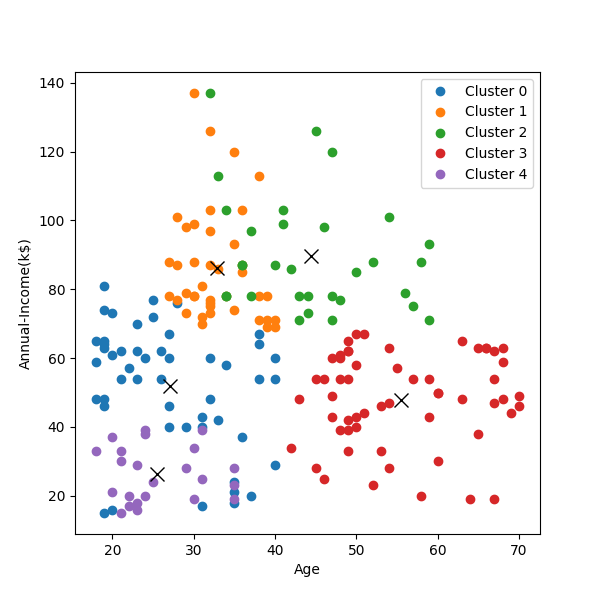
\includegraphics[width=\textwidth]{./Prob4/out/task1_rand14/images/cluster_result_k5_0_1.png}
        \caption{Age vs. Annual Income}
        \label{fig: Age vs. Annual Income k5}
    \end{minipage}
    \hfill
    \begin{minipage}{0.32\textwidth}
        \centering
        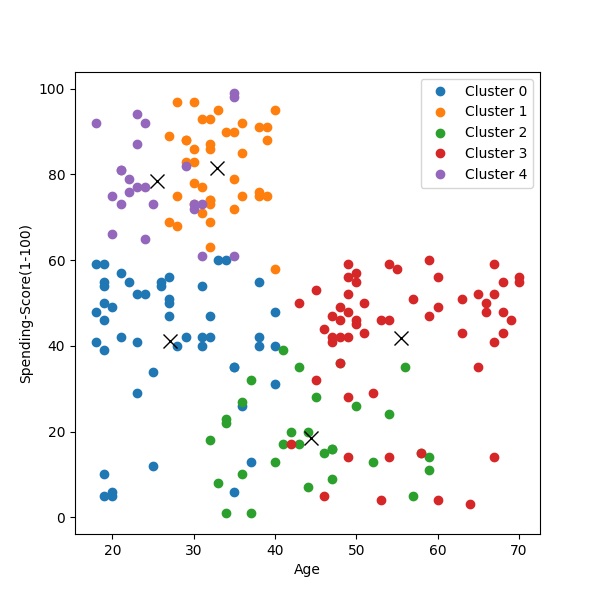
\includegraphics[width=\textwidth]{./Prob4/out/task1_rand14/images/cluster_result_k5_0_2.png}
        \caption{Age vs. Spending Score}
        \label{fig: Age vs. Spending Score k5 rand14}
    \end{minipage}
    \hfill
    \begin{minipage}{0.32\textwidth}
        \centering
        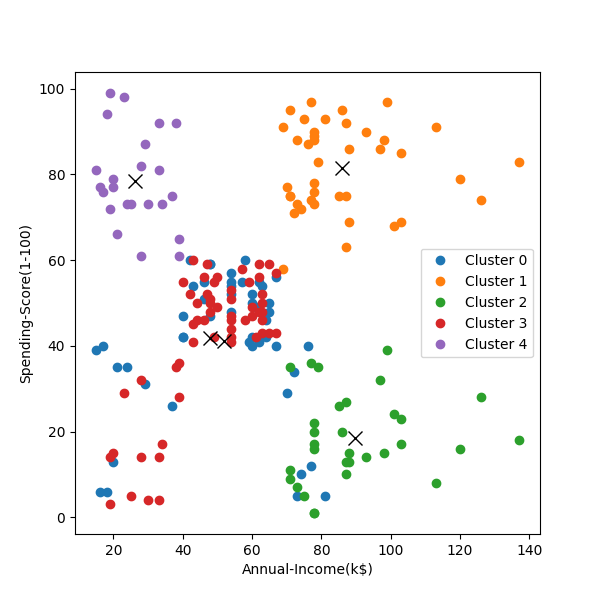
\includegraphics[width=\textwidth]{./Prob4/out/task1_rand14/images/cluster_result_k5_1_2.png}
        \caption{Annual Income vs. Spending Score}
        \label{fig: Annual Income vs. Spending Score k5 rand14}
    \end{minipage}
    \hfill
    \begin{minipage}{0.32\textwidth}
        \centering
        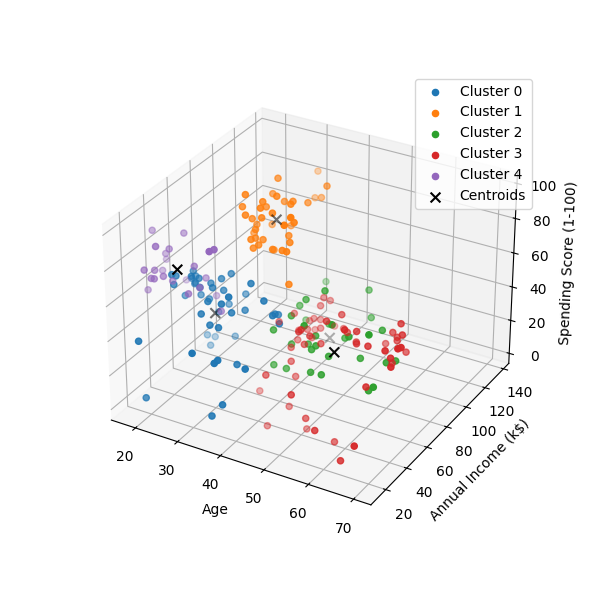
\includegraphics[width=\textwidth]{./Prob4/out/task1_rand14/images/cluster_result_k5_3d.png}
        \caption{3D Visualization}
        \label{fig: 3D Visualization k5 rand14}
    \end{minipage}
    \hfill
    \begin{minipage}{0.32\textwidth}
        \centering
        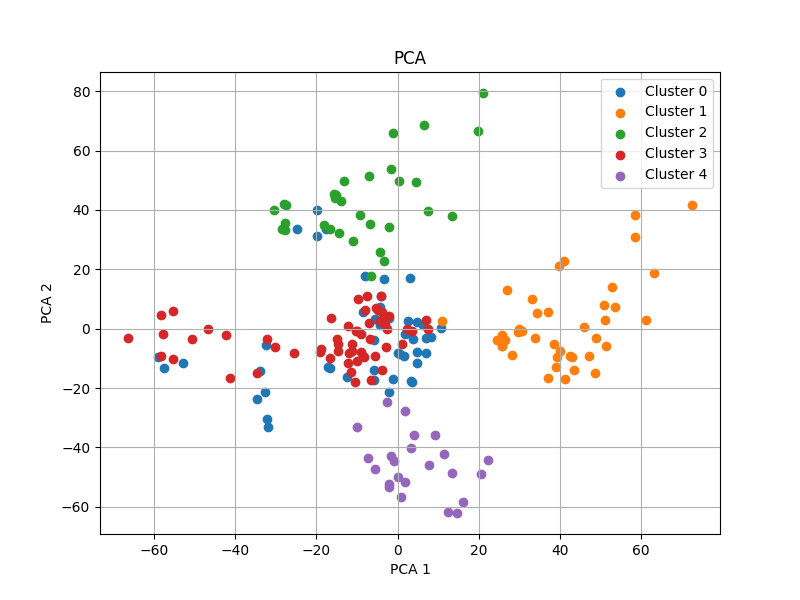
\includegraphics[width=\textwidth]{./Prob4/out/task1_rand14/images/PCA_k5.png}
        \caption{PCA Visualization}
        \label{fig: PCA Visualization k5 rand14}
    \end{minipage}
    \hfill
    \begin{minipage}{0.32\textwidth}
        \centering
        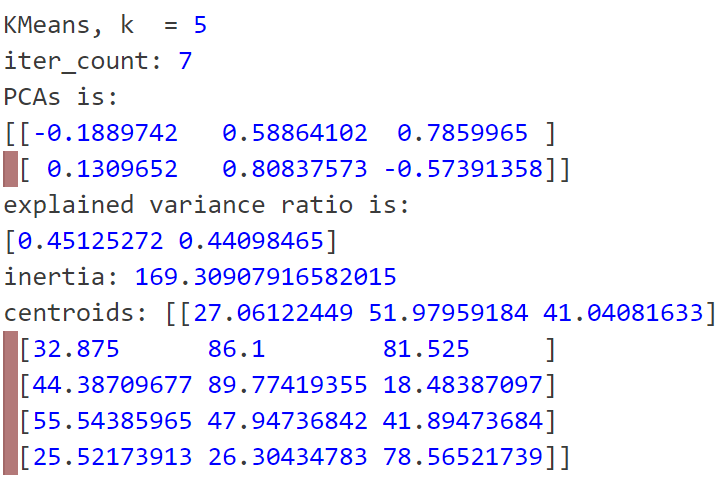
\includegraphics[width=\textwidth]{./Prob4/out/task1_rand14/log_k5.png}
        \caption{Log}
        \label{fig: log_k5.png rand14}
    \end{minipage}
\end{figure}

1.1. 簇内平方和 与 K值关系如下图所示:
\begin{figure}[H]
    \centering
    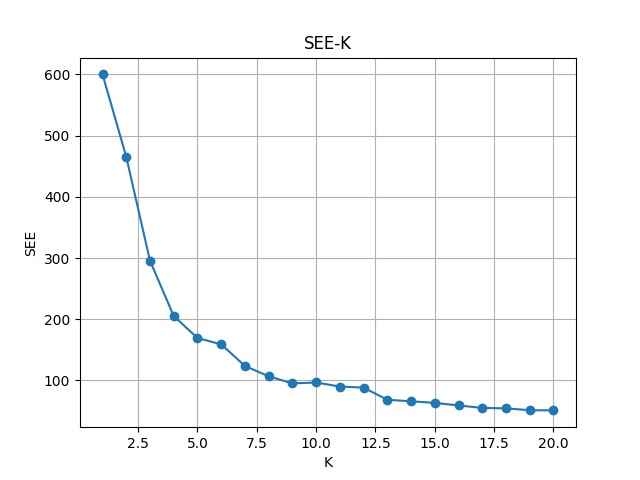
\includegraphics[width=0.5\textwidth]{./Prob4/out/task1_rand14/SEE-K.png}
    \caption{Inertia vs. K}
    \label{fig: Inertia vs. K rand14}
\end{figure}
肘部法则确定合适的k值,从图中可以看出,当K=5和7时,簇内平方和的下降速度变缓,因此选择K=5或者7。
之后我们进行了轮廓系数的计算,K=5时,轮廓系数为0.3898,稳定性0.6299;K=7时,轮廓系数为0.4223,稳定性0.7555。一定程度上说明K=7时的聚类效果更好。


K=5时,见图\ref{fig: Age vs. Spending Score k5 rand14}-图\ref{fig: log_k5.png rand14},K=7时,视图如下:
\begin{figure}[H]
    \centering
    \begin{minipage}{0.32\textwidth}
        \centering
        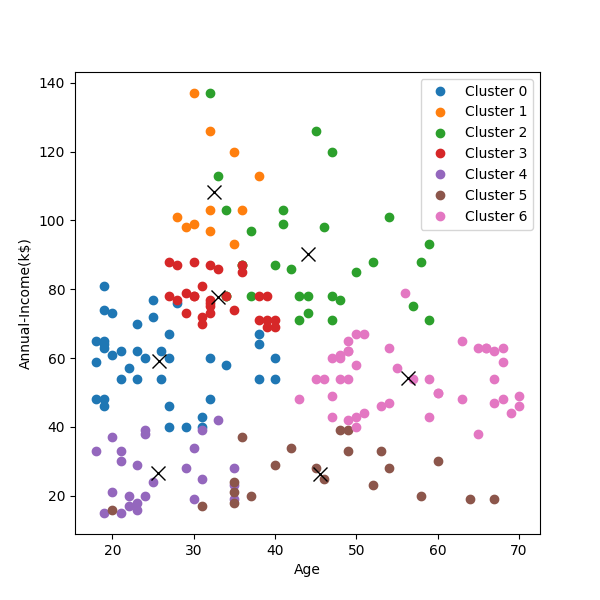
\includegraphics[width=\textwidth]{./Prob4/out/task1_rand14/images/cluster_result_k7_0_1.png}
        \caption{Age vs. Annual Income}
        \label{fig: Age vs. Annual Income k7}
    \end{minipage}
    \hfill
    \begin{minipage}{0.32\textwidth}
        \centering
        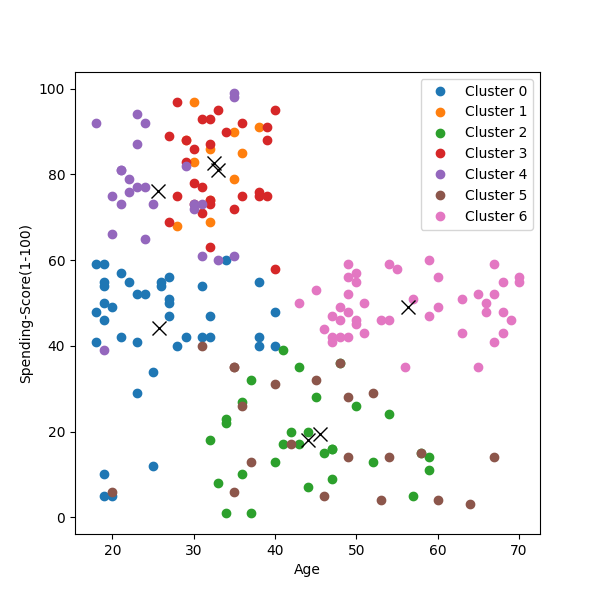
\includegraphics[width=\textwidth]{./Prob4/out/task1_rand14/images/cluster_result_k7_0_2.png}
        \caption{Age vs. Spending Score}
        \label{fig: Age vs. Spending Score k7 rand14}
    \end{minipage}
    \hfill
    \begin{minipage}{0.32\textwidth}
        \centering
        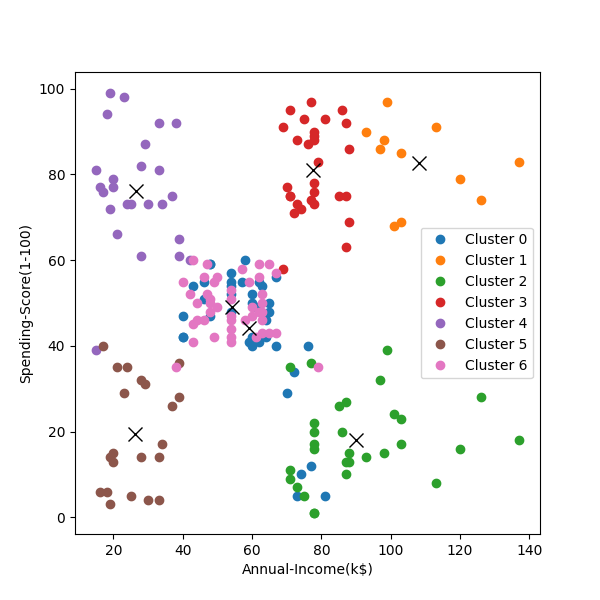
\includegraphics[width=\textwidth]{./Prob4/out/task1_rand14/images/cluster_result_k7_1_2.png}
        \caption{Annual Income vs. Spending Score}
        \label{fig: Annual Income vs. Spending Score k7 rand14}
    \end{minipage}
    \hfill
    \begin{minipage}{0.32\textwidth}
        \centering
        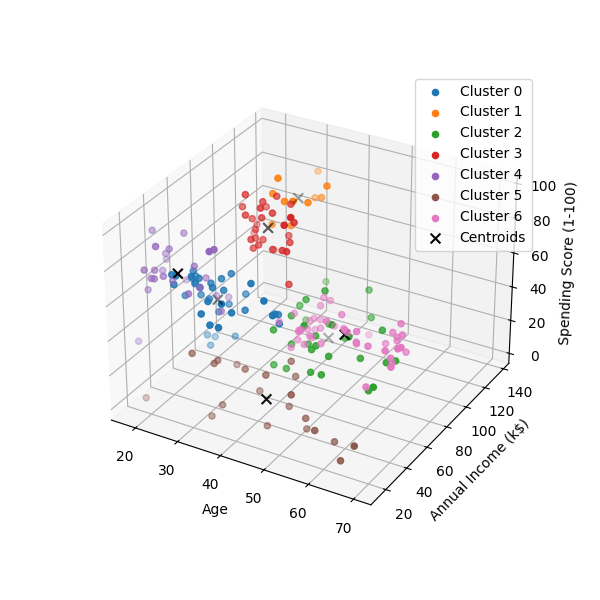
\includegraphics[width=\textwidth]{./Prob4/out/task1_rand14/images/cluster_result_k7_3d.png}
        \caption{3D Visualization}
        \label{fig: 3D Visualization k7 rand14}
    \end{minipage}
    \hfill
    \begin{minipage}{0.32\textwidth}
        \centering
        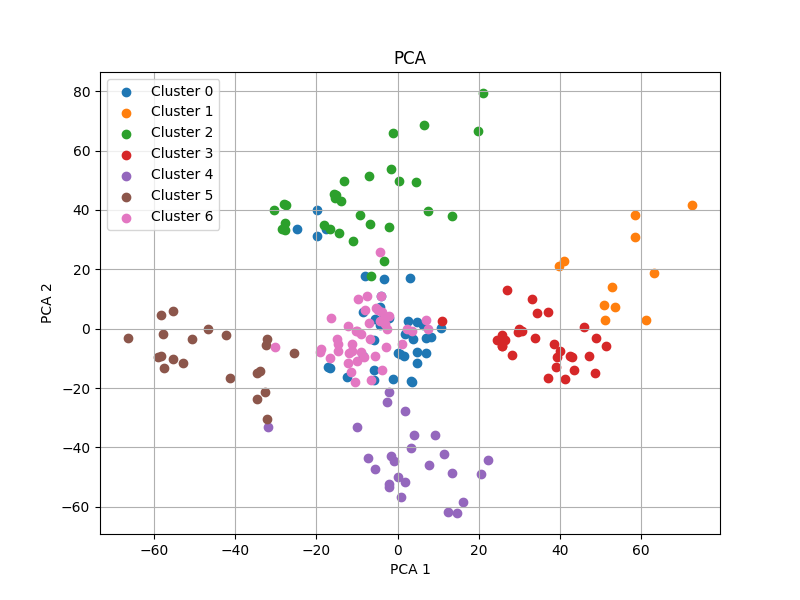
\includegraphics[width=\textwidth]{./Prob4/out/task1_rand14/images/PCA_k7.png}
        \caption{PCA Visualization}
        \label{fig: PCA Visualization k7 rand14}
    \end{minipage}
    \hfill
    \begin{minipage}{0.32\textwidth}
        \centering
        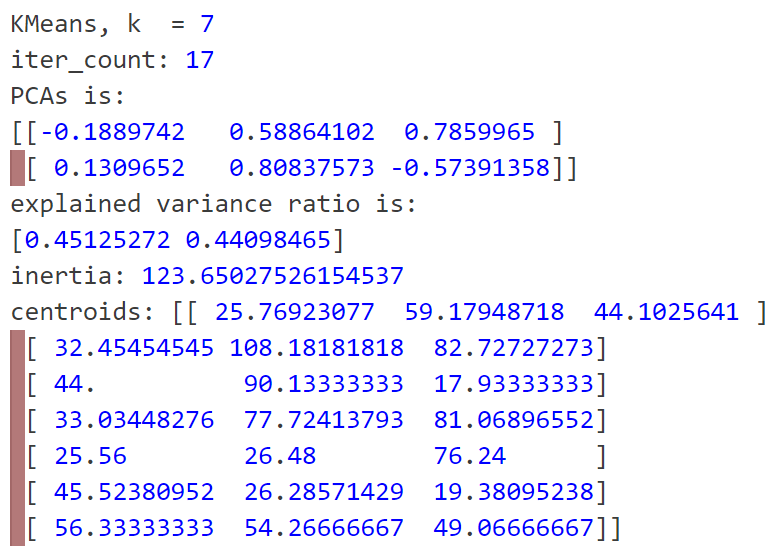
\includegraphics[width=\textwidth]{./Prob4/out/task1_rand14/log_k7.png}
        \caption{Log}
        \label{fig: log_k7.png rand14}
    \end{minipage}
\end{figure}

1.2. 简单分析每个客户群的特征 我们以 K=7 为例,对每个簇的特征进行分析:

\begin{itemize}
    \item Cluster 0: 青年到中青年;年收入中等偏下;消费积分中等,有部分消费积分较低的客户。
    \item Cluster 1: 中青年;年收入高;消费积分高;
    \item Cluster 2: 中年;年收入中等偏上,部分收入较高;消费积分较低,大部分较低。
    \item Cluster 3: 中青年;年收入中等,消费积分高。
    \item Cluster 4: 青年到中青年;年收入低,消费积分较高。
    \item Cluster 5: 几乎覆盖所有年龄段,青年较少;年收入低;消费积分较低。
    \item Cluster 6: 中老年;年收入中等偏下;消费积分中等。
\end{itemize}

1.3. 计算和分析簇内平方和(inertia) 见图\ref{fig: Inertia vs. K rand14},随着K值的增加,簇内平方和逐渐减小,但是减小速度逐渐变缓。

\vspace{3em}

2. 基于问题一的实现,我们发现随机初始化可能导致结果不稳定。请实现和分析以下改进:
\begin{itemize}
    \item 实现K-means++初始化方法(4分)
    \item 实现聚类评估指标(3分):轮廓系数(Silhouette Score)、聚类稳定性评估
    \item 对比分析(3分)
    \begin{enumerate}
        \item 比较随机初始化和K-means++的结果差异,可以通过可视化聚类图进行对比
\item 比较两种方法的稳定性
\item 分析初始化对收敛速度的影响
    \end{enumerate}
\end{itemize}

\textbf{\large 解:}

2.0. 实现K-means++初始化方法,代码见{\color{blue}./Prob4/kmeans\text{\_}pp.py中}

\begin{figure}[H]
    \centering
    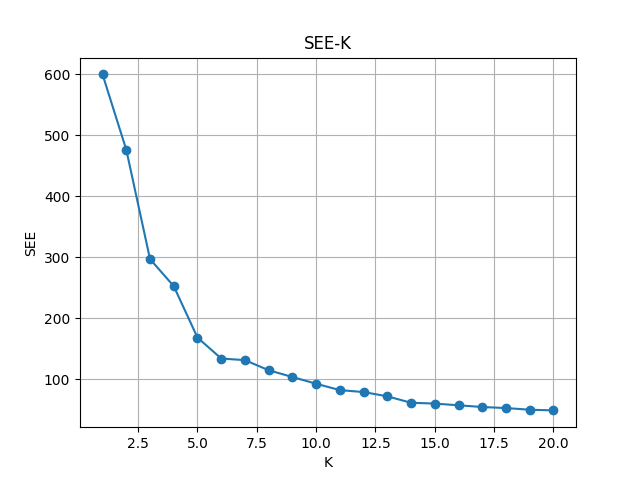
\includegraphics[width=0.5\textwidth]{./Prob4/out/task2_rand14/SEE-K.png}
    \caption{K-means++ 簇内平方和 与 K值关系}
    \label{fig: Inertia vs. K rand14 pp}
\end{figure}

根据 肘部法则,我们选取K=6,进行聚类,可视化聚类结果如下:

\begin{figure}[H]
    \centering
    \begin{minipage}{0.32\textwidth}
        \centering
        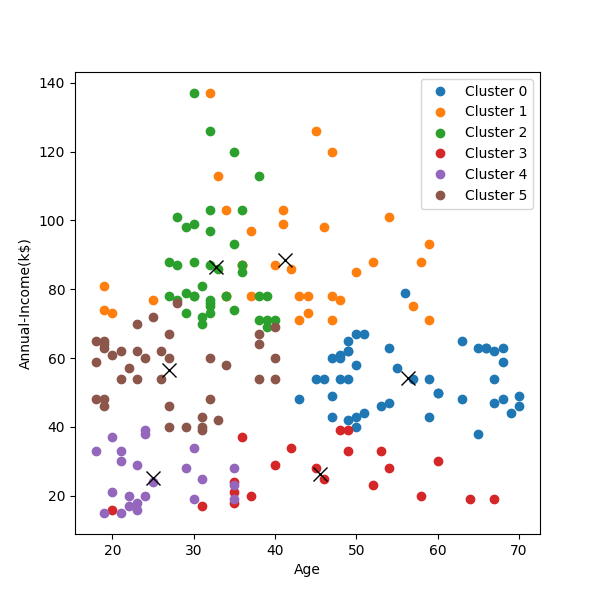
\includegraphics[width=\textwidth]{./Prob4/out/task2_rand14/images/cluster_result_k6_0_1.png}
        \caption{Age vs. Annual Income}
        \label{fig: Age vs. Annual Income k6 pp}
    \end{minipage}
    \hfill
    \begin{minipage}{0.32\textwidth}
        \centering
        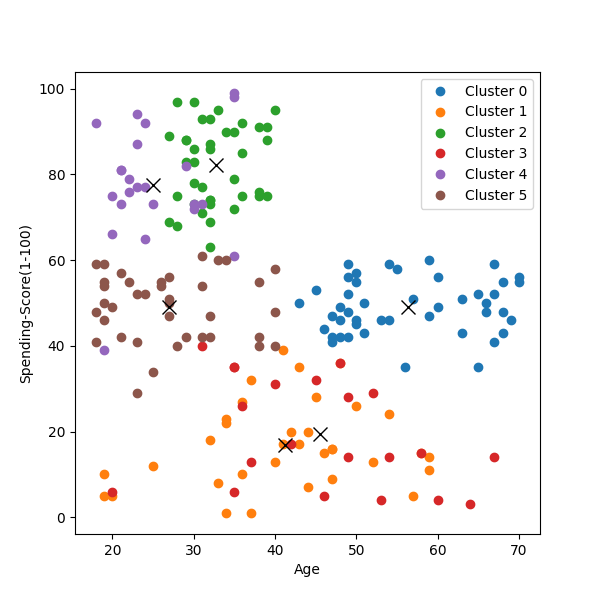
\includegraphics[width=\textwidth]{./Prob4/out/task2_rand14/images/cluster_result_k6_0_2.png}
        \caption{Age vs. Spending Score}
        \label{fig: Age vs. Spending Score k6 rand14 pp}
    \end{minipage}
    \hfill
    \begin{minipage}{0.32\textwidth}
        \centering
        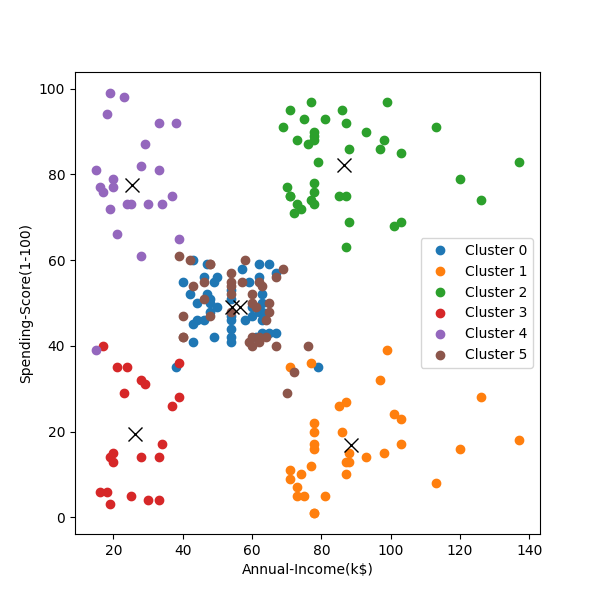
\includegraphics[width=\textwidth]{./Prob4/out/task2_rand14/images/cluster_result_k6_1_2.png}
        \caption{Annual Income vs. Spending Score}
        \label{fig: Annual Income vs. Spending Score k6 rand14 pp}
    \end{minipage}
    \hfill
    \begin{minipage}{0.32\textwidth}
        \centering
        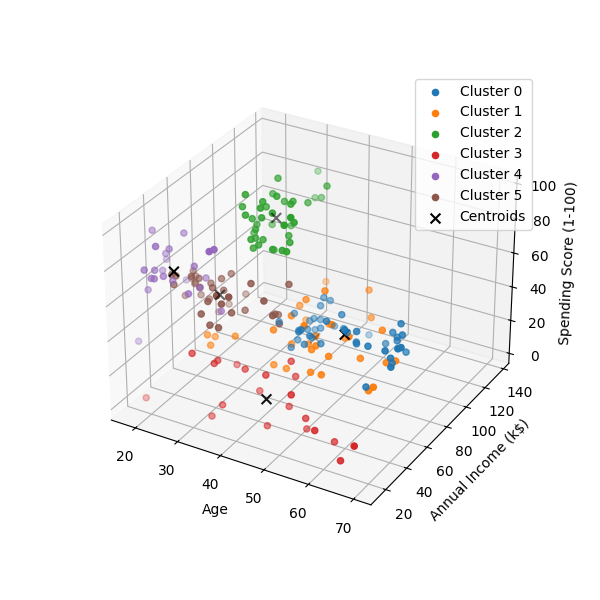
\includegraphics[width=\textwidth]{./Prob4/out/task2_rand14/images/cluster_result_k6_3d.png}
        \caption{3D Visualization}
        \label{fig: 3D Visualization k6 rand14 pp}
    \end{minipage}
    \hfill
    \begin{minipage}{0.32\textwidth}
        \centering
        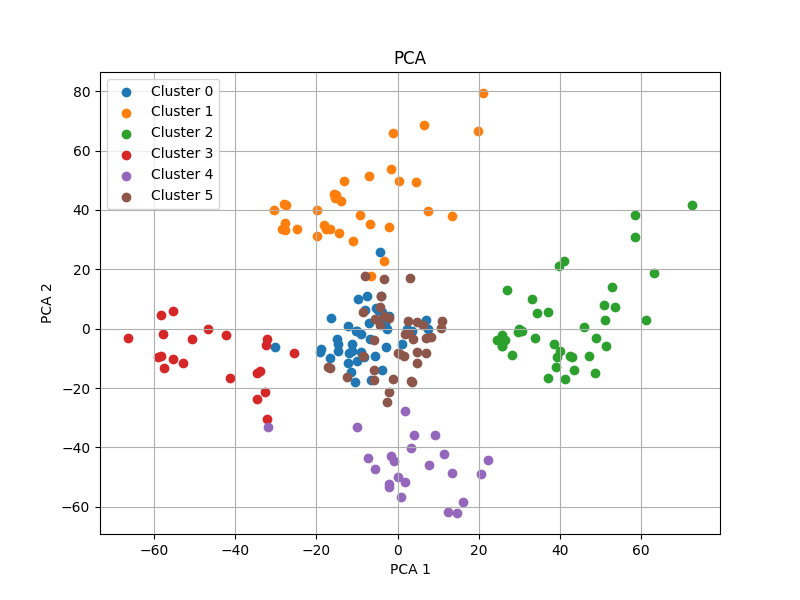
\includegraphics[width=\textwidth]{./Prob4/out/task2_rand14/images/PCA_k6.png}
        \caption{PCA Visualization}
        \label{fig: PCA Visualization k6 rand14 pp}
    \end{minipage}
    \hfill
    \begin{minipage}{0.32\textwidth}
        \centering
        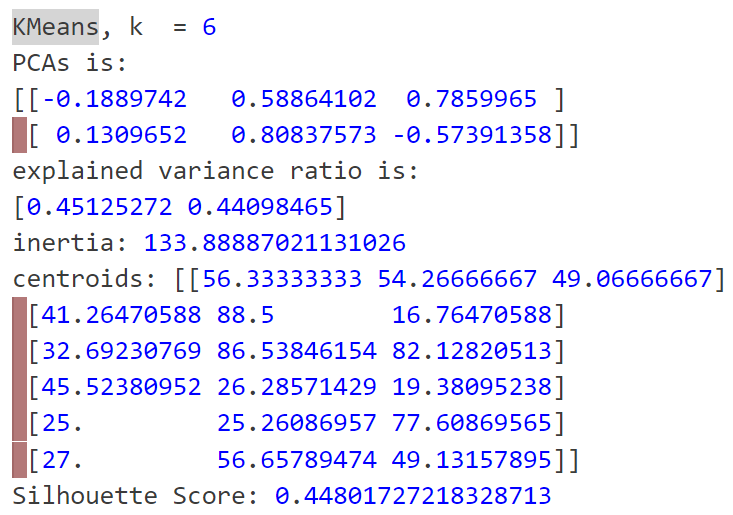
\includegraphics[width=\textwidth]{./Prob4/out/task2_rand14/log_k6.png}
        \caption{Log}
        \label{fig: log_k6.png rand14 pp}
    \end{minipage}
\end{figure}

2.1. 实现聚类评估指标,(轮廓系数 (Silhouette Score)、聚类稳定性评估) 

代码见 {\color{blue}Prob4/utils.py}

轮廓系数的输出在log中。表如下
\begin{table}[H]
    \centering
    \begin{tabular}{|c|c|}
        \hline
        K & Silhouette Score  \\
        \hline
        2 & 0.3251  \\
        3 & 0.3115  \\
        4 & 0.3041  \\
        5 & 0.4162  \\
        6 & 0.4480  \\
        7 & 0.3959  \\
        8 & 0.3563  \\
        9 & 0.3304  \\
        10 & 0.3108  \\
        11 & 0.3053  \\
        12 & 0.2993  \\
        13 & 0.2933  \\
        14 & 0.3114  \\
        15 & 0.3212  \\
        16 & 0.3296  \\
        17 & 0.3060  \\
        18 & 0.2884  \\
        19 & 0.2745  \\
        20 & 0.2699  \\
        \hline
    \end{tabular}
    \caption{Silhouette Score}
\end{table}

稳定性见下图\ref{fig: Kmeans vs. Kmeans++ Stability 50rounds}。

2.2. 对比分析

2.2.1. 以 K = 6,randseed = 14 为例,对比结果差异,可视化图如下:

\begin{figure}[H]
    \centering
    \begin{minipage}{0.32\textwidth}
        \centering
        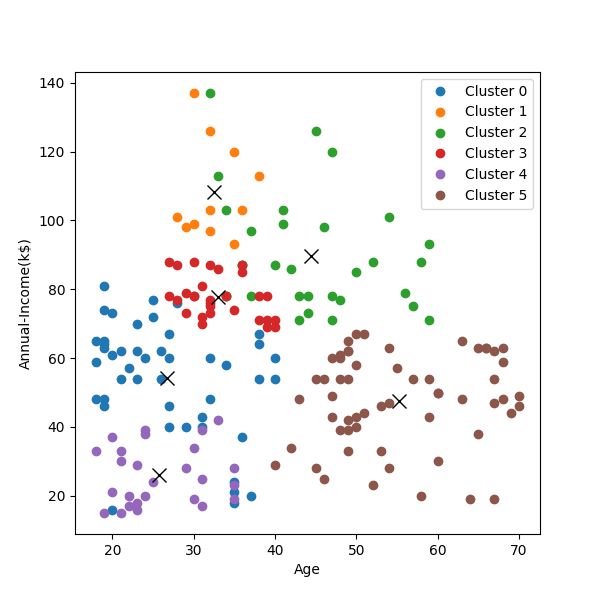
\includegraphics[width=\textwidth]{./Prob4/out/task1_rand14/images/cluster_result_k6_0_1.png}
        \caption{Kmeans: Age vs. Income}
        \label{fig: Age vs. Annual Income k6 com}
    \end{minipage}
    \hfill
    \begin{minipage}{0.32\textwidth}
        \centering
        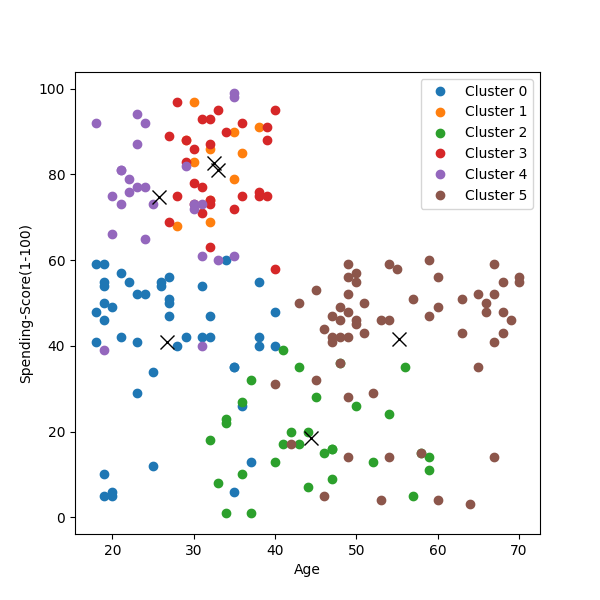
\includegraphics[width=\textwidth]{./Prob4/out/task1_rand14/images/cluster_result_k6_0_2.png}
        \caption{Kmeans: Age vs. Spending}
        \label{fig: Age vs. Spending Score k6 rand14 com}
    \end{minipage}
    \hfill
    \begin{minipage}{0.32\textwidth}
        \centering
        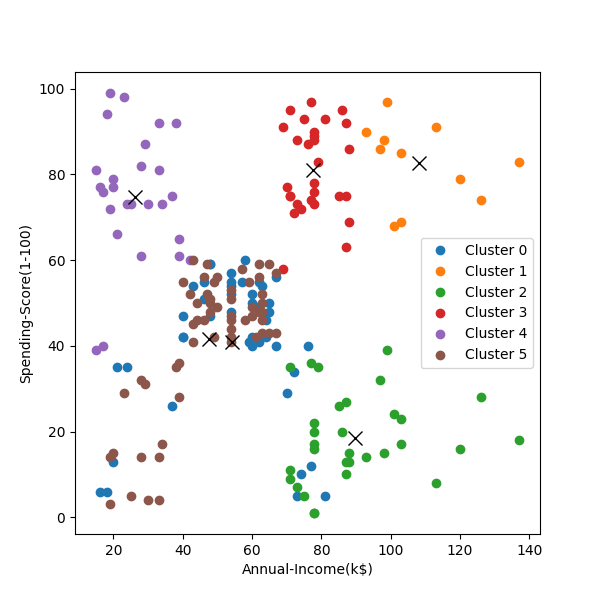
\includegraphics[width=\textwidth]{./Prob4/out/task1_rand14/images/cluster_result_k6_1_2.png}
        \caption{Kmeans: Income vs. Spending}
        \label{fig: Annual Income vs. Spending Score k6 rand14 com}
    \end{minipage}
    \hfill
    \begin{minipage}{0.32\textwidth}
        \centering
        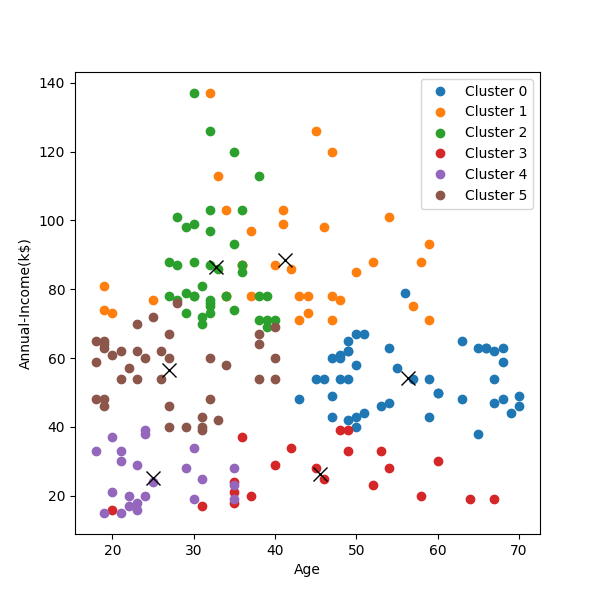
\includegraphics[width=\textwidth]{./Prob4/out/task2_rand14/images/cluster_result_k6_0_1.png}
        \caption{Kmeans++: Age vs. Income}
        \label{fig: Age vs. Annual Income k6 pp com}
    \end{minipage}
    \hfill
    \begin{minipage}{0.32\textwidth}
        \centering
        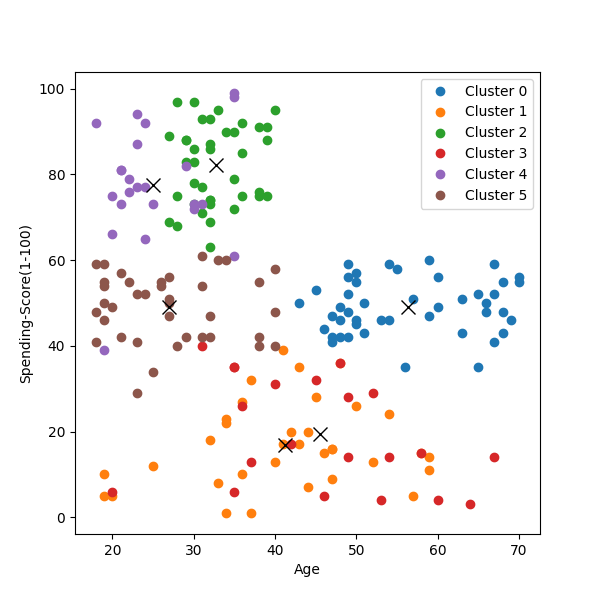
\includegraphics[width=\textwidth]{./Prob4/out/task2_rand14/images/cluster_result_k6_0_2.png}
        \caption{Kmeans++: Age vs. Spending}
        \label{fig: Age vs. Spending Score k6 rand14 pp com}
    \end{minipage}
    \hfill
    \begin{minipage}{0.32\textwidth}
        \centering
        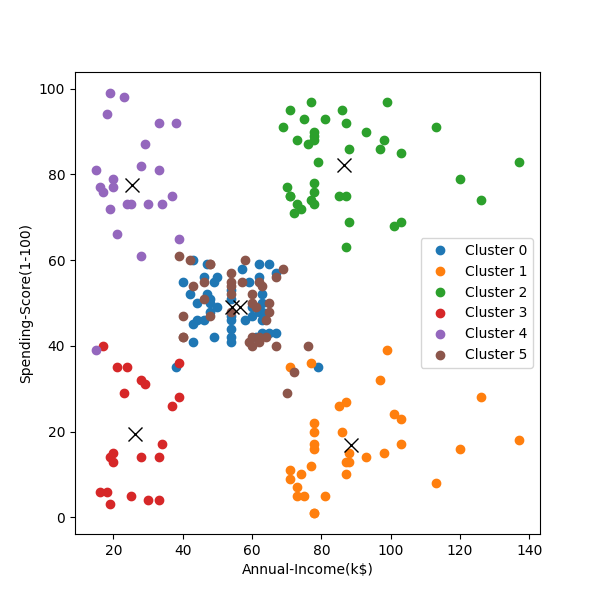
\includegraphics[width=\textwidth]{./Prob4/out/task2_rand14/images/cluster_result_k6_1_2.png}
        \caption{Kmeans++: Income vs. Spending}
        \label{fig: Annual Income vs. Spending Score k6 rand14 pp com}
    \end{minipage}
    \hfill
\end{figure}

从图中可以看出,
随机初始化细分了高收入高积分人群,即图\ref{fig: Age vs. Annual Income k6 com}-图\ref{fig: Annual Income vs. Spending Score k6 rand14 com}中的Cluster1和Cluster3,
但是对于中低收入中低积分的人群,即图\ref{fig: Age vs. Annual Income k6 com}-图\ref{fig: Annual Income vs. Spending Score k6 rand14 com}中的Cluster 0和Cluster 5的分类明显不当;
而Kmeans++,则将中低收入中低积分的人群细分为图\ref{fig: Age vs. Annual Income k6 pp com}-图\ref{fig: Annual Income vs. Spending Score k6 rand14 pp com}中的Cluster 0, Cluster 3 和 Cluster5,
并把一部分中等收入群体分类到中高收入人群(图\ref{fig: Age vs. Annual Income k6 pp com}-图\ref{fig: Annual Income vs. Spending Score k6 rand14 pp com}中的Cluster 1)中,分类更加合理。

\begin{figure}[H]
    \centering
    \begin{minipage}{0.45\textwidth}
        \centering
        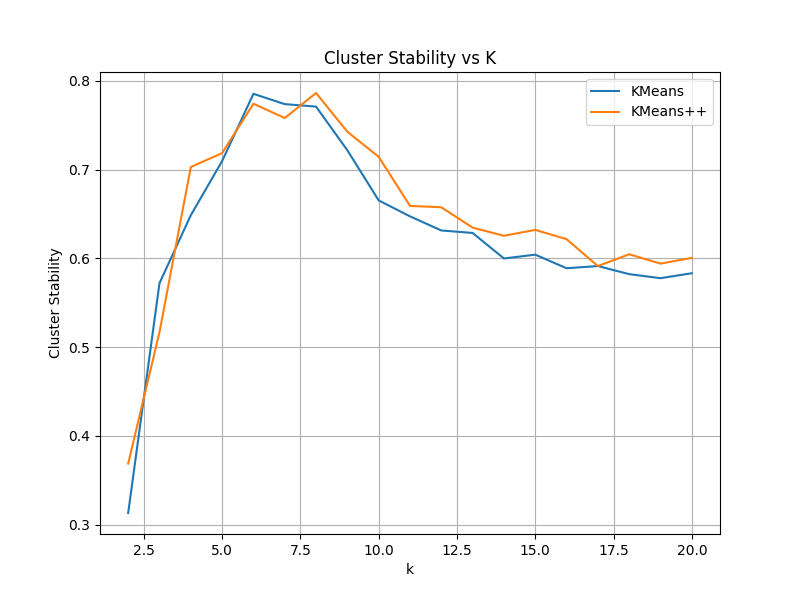
\includegraphics[width=\textwidth]{./Prob4/out/task_2_2/stabilities_k20.png}
        \caption{Stability vs. K}
        \label{fig: Kmeans vs. Kmeans++ Stability 50rounds}
    \end{minipage}
    \hfill
    \begin{minipage}{0.45\textwidth}
        \centering
        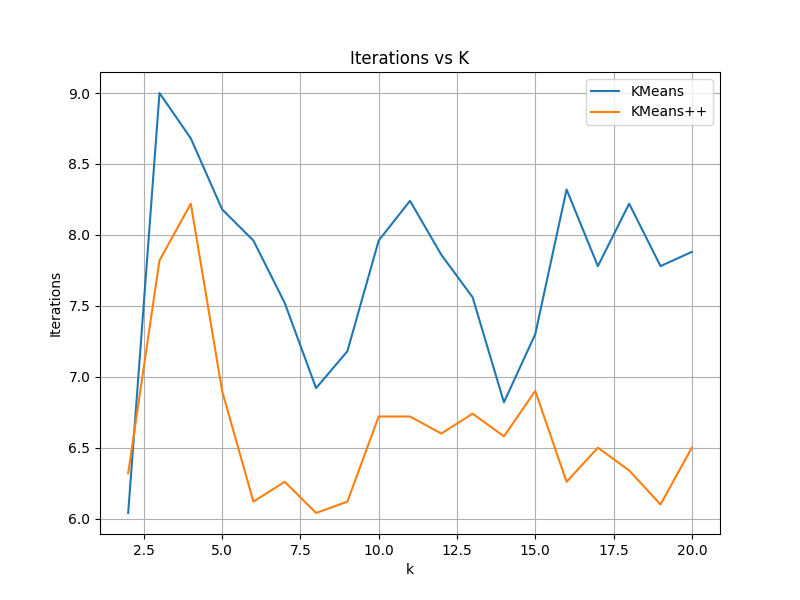
\includegraphics[width=\textwidth]{./Prob4/out/task_2_2/iters_k20.png}
        \caption{iters vs. K}
        \label{fig: Kmeans vs. Kmeans++ iters 50rounds}
    \end{minipage}
    \hfill
\end{figure}

2.2.2. 比较两种方法的稳定性:

我们采取了50轮的随机实验(不固定随机种子),计算了两种初始化方法的稳定性,并取平均值,见图\ref{fig: Kmeans vs. Kmeans++ Stability 50rounds}。可见,平均来看两者稳定性相差不大。

2.2.3. 分析初始化对收敛速度的影响:

我们采取了50轮的随机实验(不固定随机种子),计算了两种初始化方法的迭代轮数,并取平均值,见图\ref{fig: Kmeans vs. Kmeans++ iters 50rounds}。可见,Kmeans++方法的收敛速度更快。

\vspace{3em}

3. 在实际业务中,不同特征的重要性可能不同,且某些客户群可能需要大小相近。请实现带权重和大小约束的改进版本:
\begin{itemize}
    \item 实现带约束的聚类算法,需要支持特征加权和簇大小约束(4 points)
    \item 在以下两个场景下重新进行实验:收入特征权重加倍,限制每个客户群至少包含20\%的客户, 绘制聚类结果(6 points)
\end{itemize}

\textbf{\large 解:}

3.1 实现带约束的聚类算法,代码见 {\color{blue}Prob4/kmeans\text{\_}cons.py} 和 {\color{blue}Prob4/kmeans\text{\_}mcons.py}

3.2 在以下两个场景下重新进行实验,绘制聚类结果:

我们固定了随机种子为14,以保证结果的可重复性。

3.2.1 收入特征权重加倍

\begin{figure}[H]
    \centering
    \begin{minipage}{0.32\textwidth}
        \centering
        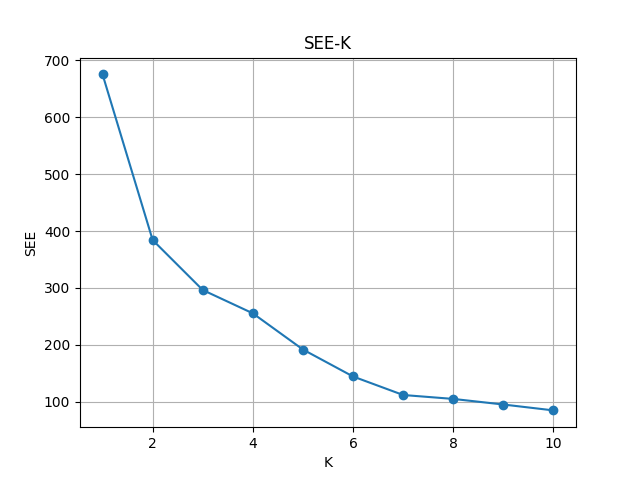
\includegraphics[width=\textwidth]{./Prob4/out/task3_1_com/SEE-K.png}
        \caption{Inertia vs. K}
        \label{fig: Inertia vs. K com}
    \end{minipage}
    \hfill
    \begin{minipage}{0.32\textwidth}
        \centering
        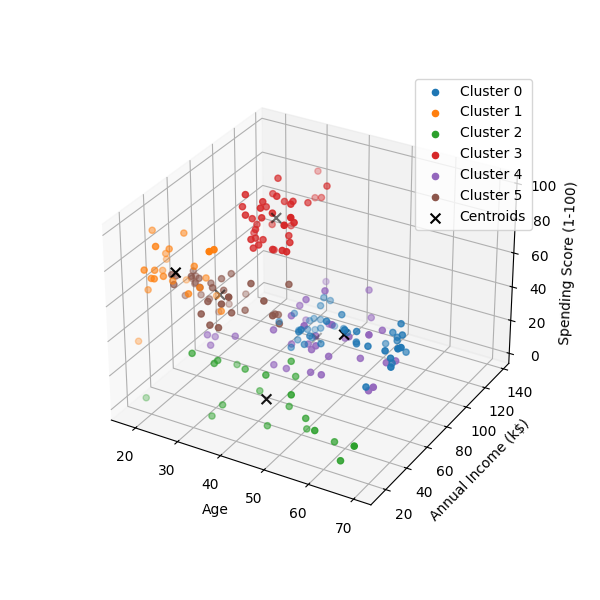
\includegraphics[width=\textwidth]{./Prob4/out/task3_1_com/images/cluster_result_k6_3d.png}
        \caption{3D Visualization}
        \label{fig: 3D k6 com con w}
    \end{minipage}
    \hfill
    \begin{minipage}{0.32\textwidth}
        \centering
        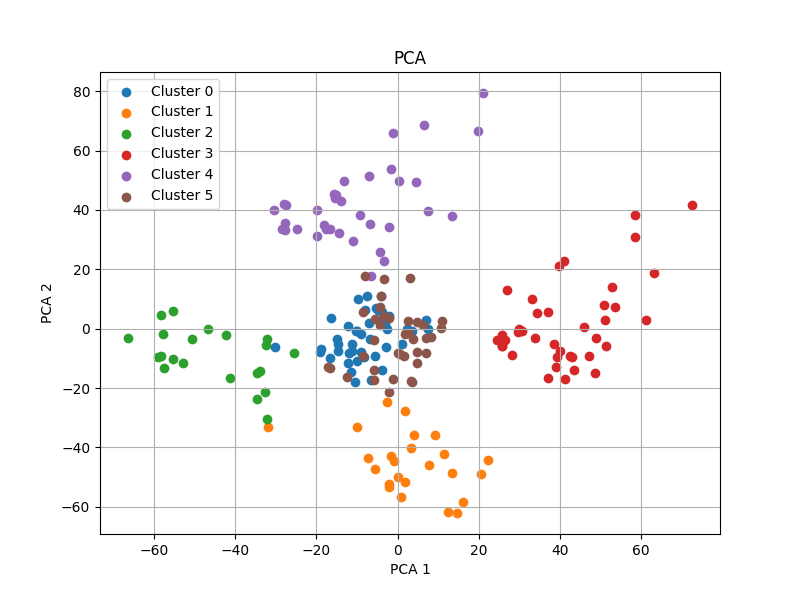
\includegraphics[width=\textwidth]{./Prob4/out/task3_1_com/images/PCA_k6.png}
        \caption{PCA Visualization}
        \label{PCA k6 com con w}
    \end{minipage}
    \hfill
    \begin{minipage}{0.32\textwidth}
        \centering
        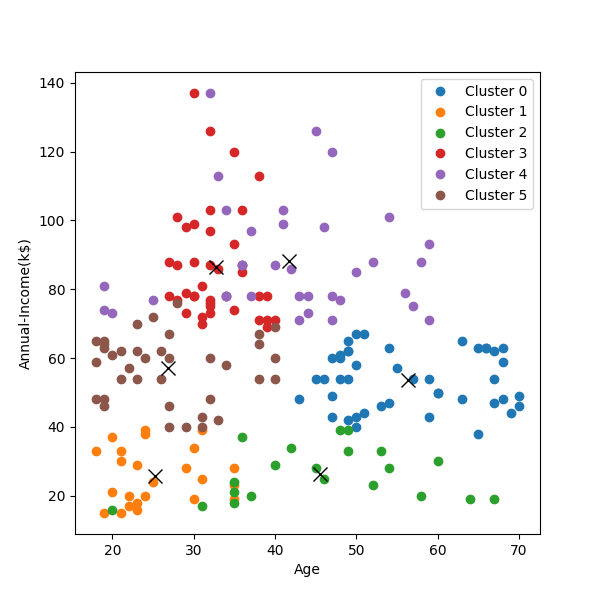
\includegraphics[width=\textwidth]{./Prob4/out/task3_1_com/images/cluster_result_k6_0_1.png}
        \caption{Age vs. Income}
        \label{fig: Age vs. Annual Income k6 com con w}
    \end{minipage}
    \hfill
    \begin{minipage}{0.32\textwidth}
        \centering
        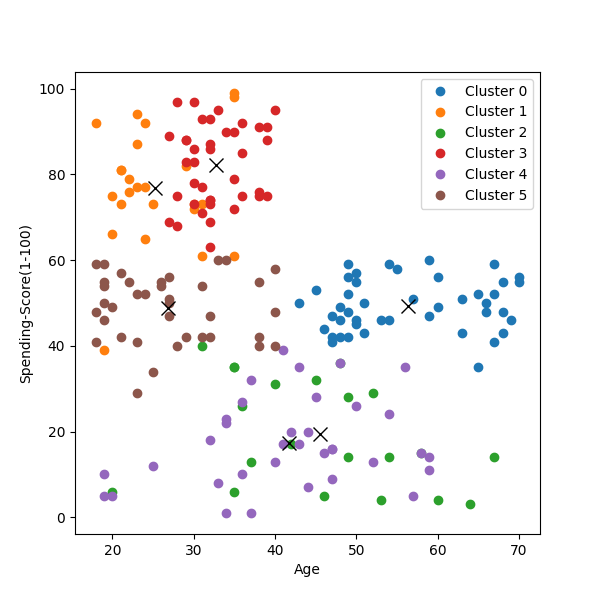
\includegraphics[width=\textwidth]{./Prob4/out/task3_1_com/images/cluster_result_k6_0_2.png}
        \caption{Age vs. Spending}
        \label{fig: Age vs. Spending Score k6 com con w}
    \end{minipage}
    \hfill
    \begin{minipage}{0.32\textwidth}
        \centering
        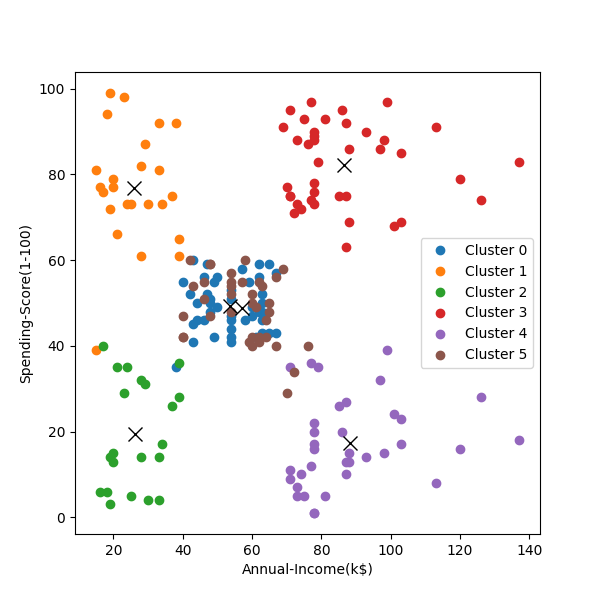
\includegraphics[width=\textwidth]{./Prob4/out/task3_1_com/images/cluster_result_k6_1_2.png}
        \caption{Income vs. Spending}
        \label{fig: Annual Income vs. Spending Score k6 com con w}
    \end{minipage}
    \hfill
\end{figure}

3.2.2 限制每个客户群至少包含20\%的客户

查阅资料,限制最小簇的实现可以使用最小成本流算法,代码见 {\color{blue}Prob4/kmeans\text{\_}cons.py}。K=4和5的图片如下:

\begin{figure}[H]
    \centering
    \begin{minipage}{0.32\textwidth}
        \centering
        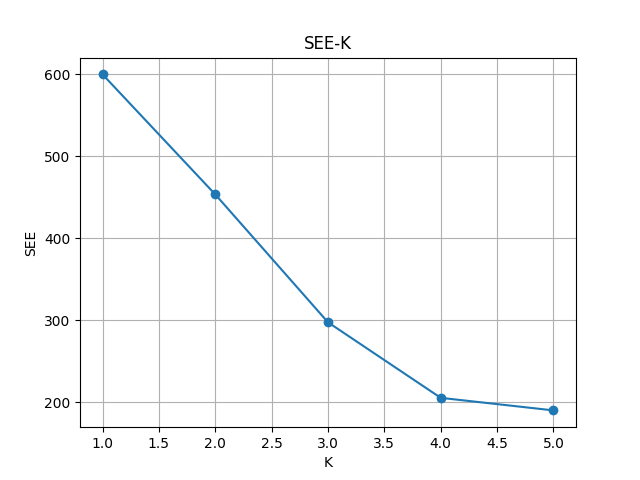
\includegraphics[width=\textwidth]{./Prob4/out/task3_2_com/SEE-K.png}
        \caption{Inertia vs. K}
        \label{fig: Inertia vs. K com min20 2}
    \end{minipage}
    \hfill
    \begin{minipage}{0.32\textwidth}
        \centering
        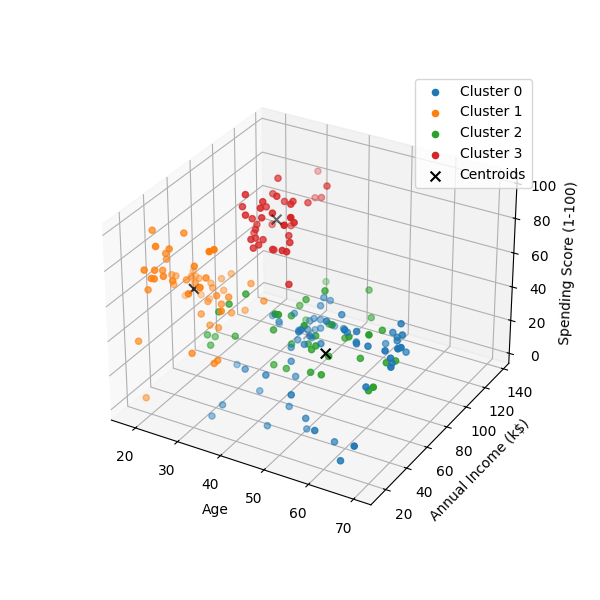
\includegraphics[width=\textwidth]{./Prob4/out/task3_2_com/images/cluster_result_k4_3d.png}
        \caption{3D Visualization}
        \label{fig: 3D k4 com con min20}
    \end{minipage}
    \hfill
    \begin{minipage}{0.32\textwidth}
        \centering
        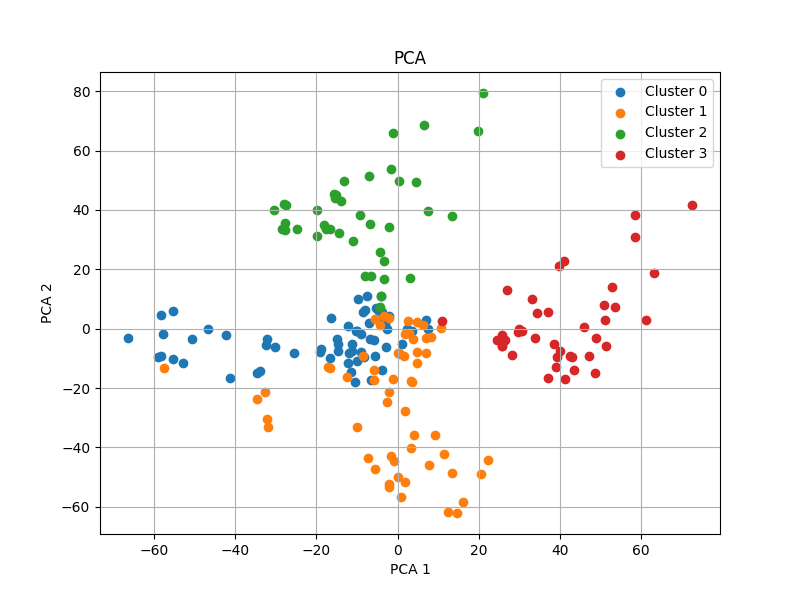
\includegraphics[width=\textwidth]{./Prob4/out/task3_2_com/images/PCA_k4.png}
        \caption{PCA Visualization}
        \label{PCA k4 com con min20}
    \end{minipage}
    \hfill
    \begin{minipage}{0.32\textwidth}
        \centering
        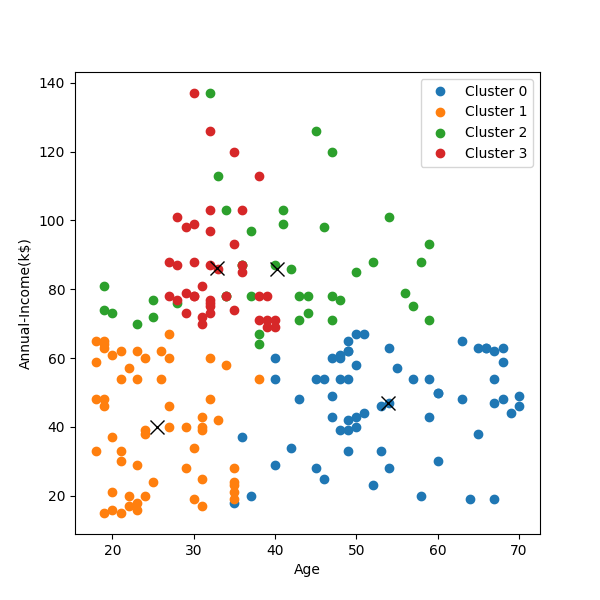
\includegraphics[width=\textwidth]{./Prob4/out/task3_2_com/images/cluster_result_k4_0_1.png}
        \caption{Age vs. Income}
        \label{fig: Age vs. Annual Income k4 com con min20}
    \end{minipage}
    \hfill
    \begin{minipage}{0.32\textwidth}
        \centering
        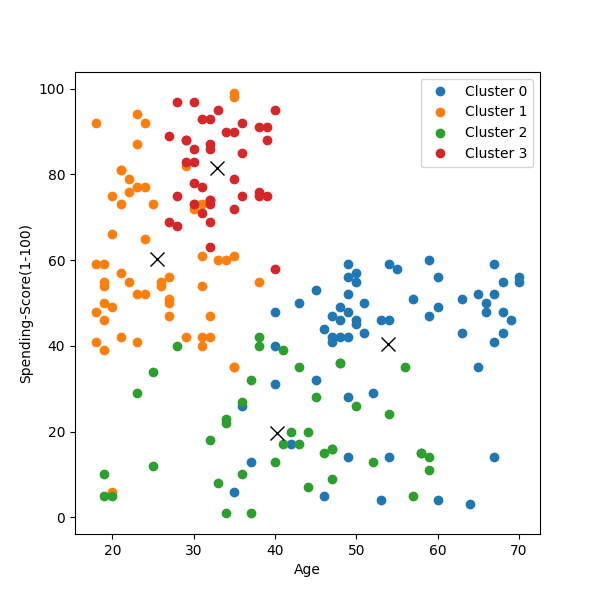
\includegraphics[width=\textwidth]{./Prob4/out/task3_2_com/images/cluster_result_k4_0_2.png}
        \caption{Age vs. Spending}
        \label{fig: Age vs. Spending Score k4 com con min20}
    \end{minipage}
    \hfill
    \begin{minipage}{0.32\textwidth}
        \centering
        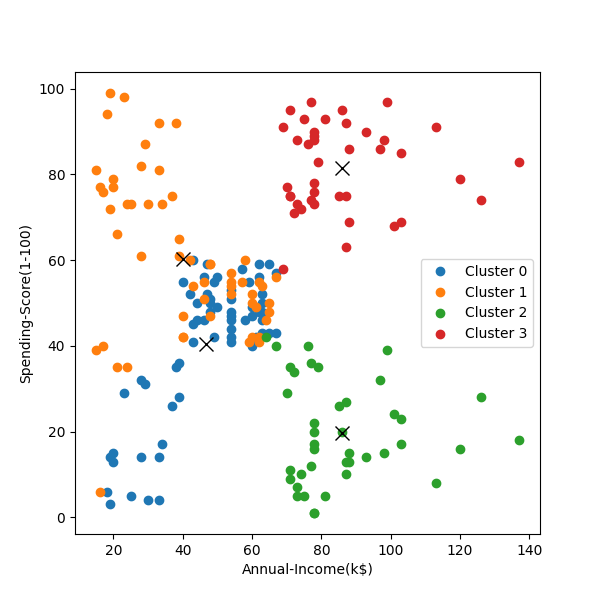
\includegraphics[width=\textwidth]{./Prob4/out/task3_2_com/images/cluster_result_k4_1_2.png}
        \caption{Income vs. Spending}
        \label{fig: Annual Income vs. Spending Score k4 com con min20}
    \end{minipage}
    \hfill
\end{figure}

\begin{figure}[H]
    \centering
    \begin{minipage}{0.32\textwidth}
        \centering
        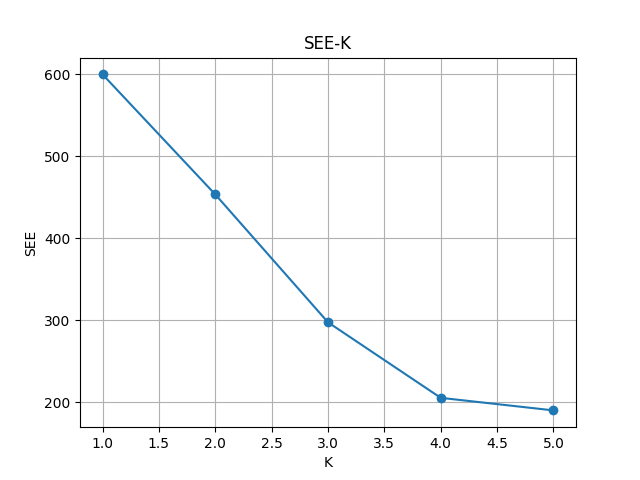
\includegraphics[width=\textwidth]{./Prob4/out/task3_2_com/SEE-K.png}
        \caption{Inertia vs. K}
        \label{fig: Inertia vs. K com min20}
    \end{minipage}
    \hfill
    \begin{minipage}{0.32\textwidth}
        \centering
        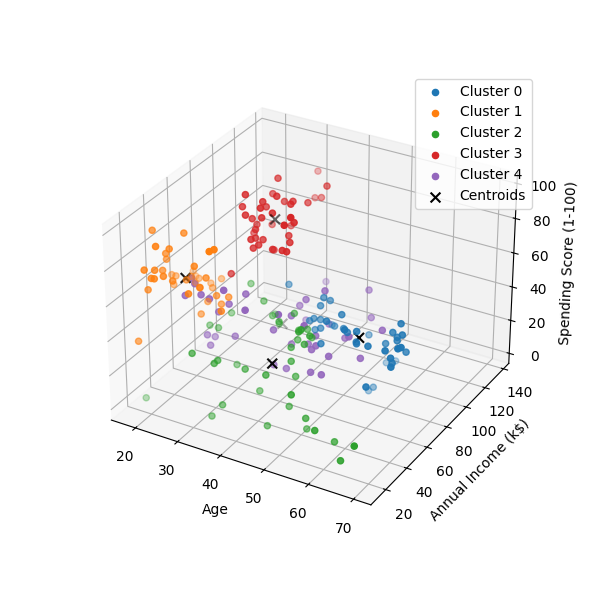
\includegraphics[width=\textwidth]{./Prob4/out/task3_2_com/images/cluster_result_k5_3d.png}
        \caption{3D Visualization}
        \label{fig: 3D k5 com con min20}
    \end{minipage}
    \hfill
    \begin{minipage}{0.32\textwidth}
        \centering
        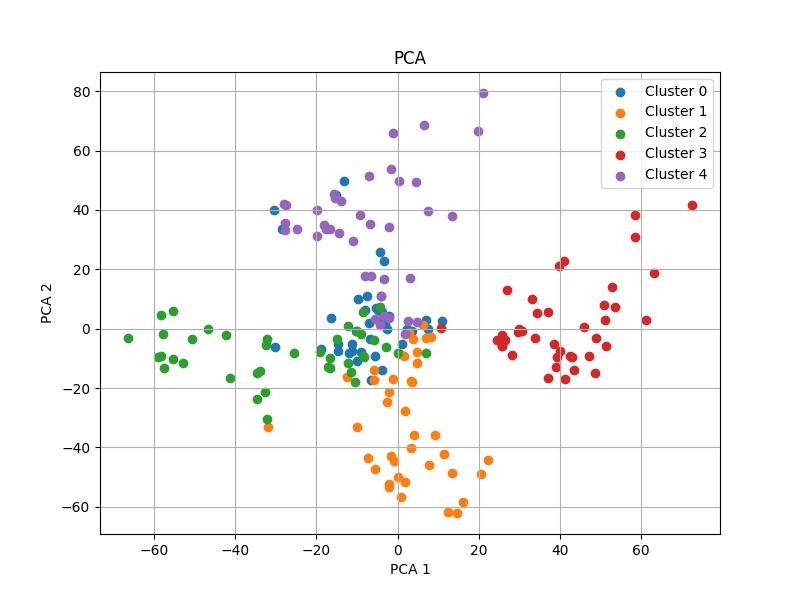
\includegraphics[width=\textwidth]{./Prob4/out/task3_2_com/images/PCA_k5.png}
        \caption{PCA Visualization}
        \label{PCA k5 com con min20}
    \end{minipage}
    \hfill
    \begin{minipage}{0.32\textwidth}
        \centering
        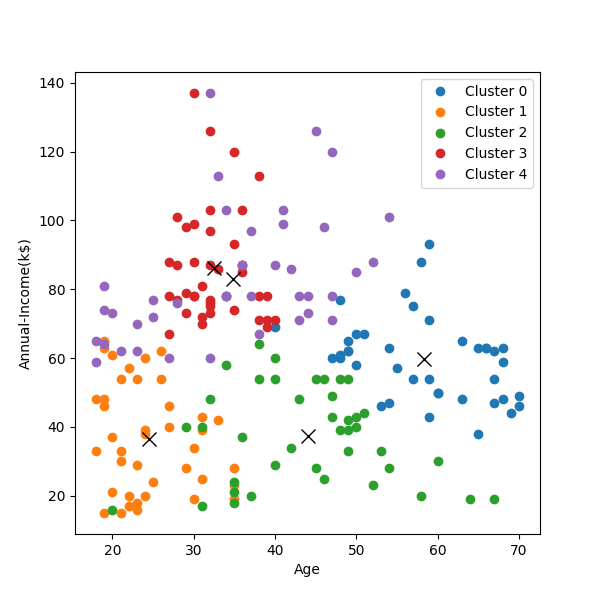
\includegraphics[width=\textwidth]{./Prob4/out/task3_2_com/images/cluster_result_k5_0_1.png}
        \caption{Age vs. Income}
        \label{fig: Age vs. Annual Income k5 com con min20}
    \end{minipage}
    \hfill
    \begin{minipage}{0.32\textwidth}
        \centering
        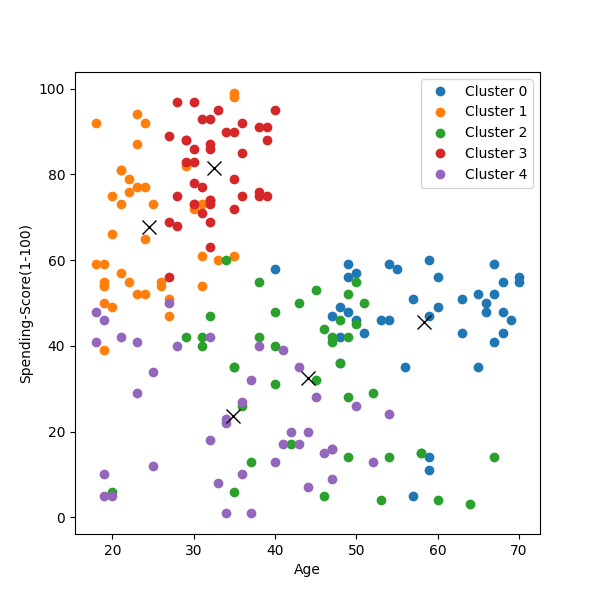
\includegraphics[width=\textwidth]{./Prob4/out/task3_2_com/images/cluster_result_k5_0_2.png}
        \caption{Age vs. Spending}
        \label{fig: Age vs. Spending Score k5 com con min20}
    \end{minipage}
    \hfill
    \begin{minipage}{0.32\textwidth}
        \centering
        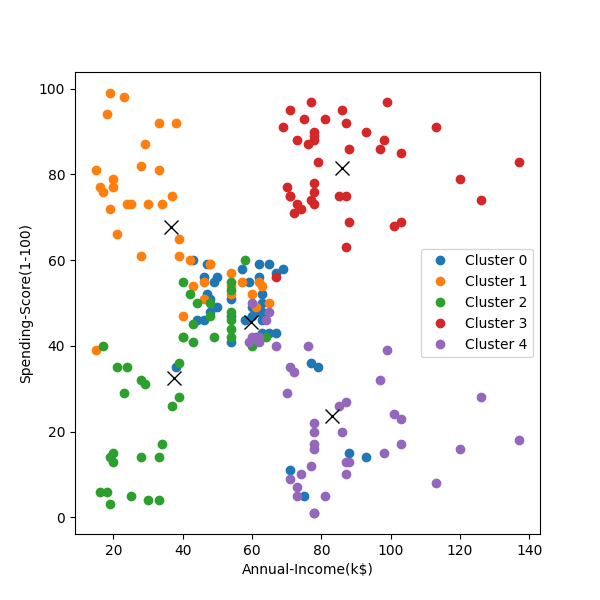
\includegraphics[width=\textwidth]{./Prob4/out/task3_2_com/images/cluster_result_k5_1_2.png}
        \caption{Income vs. Spending}
        \label{fig: Annual Income vs. Spending Score k5 com con min20}
    \end{minipage}
    \hfill
\end{figure}

此外,在摸索过程中,我实现了一个不如最小成本流的贪心近似算法,代码见 {\color{blue}Prob4/kmeans\text{\_}mcons.py}。图片如下:

\begin{figure}[H]
    \centering
    \begin{minipage}{0.32\textwidth}
        \centering
        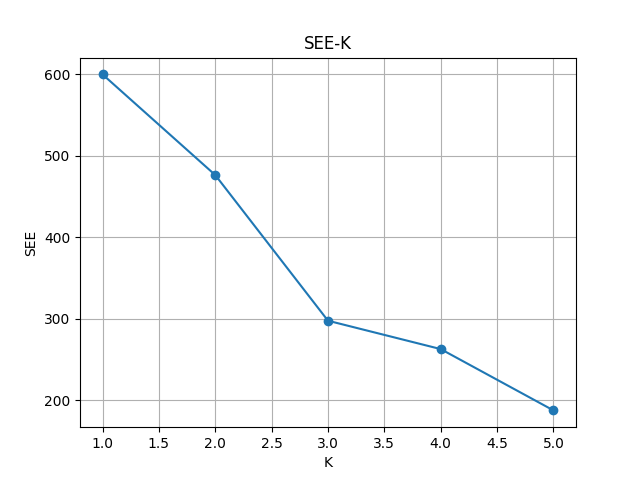
\includegraphics[width=\textwidth]{./Prob4/out/task3_2_mcom2/SEE-K.png}
        \caption{Inertia vs. K}
        \label{fig: Inertia vs. K mcom min20}
    \end{minipage}
    \hfill
    \begin{minipage}{0.32\textwidth}
        \centering
        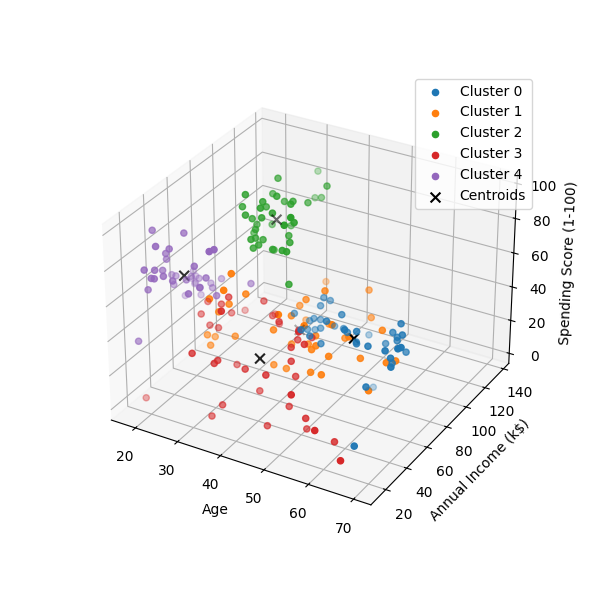
\includegraphics[width=\textwidth]{./Prob4/out/task3_2_mcom2/images/cluster_result_k5_3d.png}
        \caption{3D Visualization}
        \label{fig: 3D k5 mcom2 con min20}
    \end{minipage}
    \hfill
    \begin{minipage}{0.32\textwidth}
        \centering
        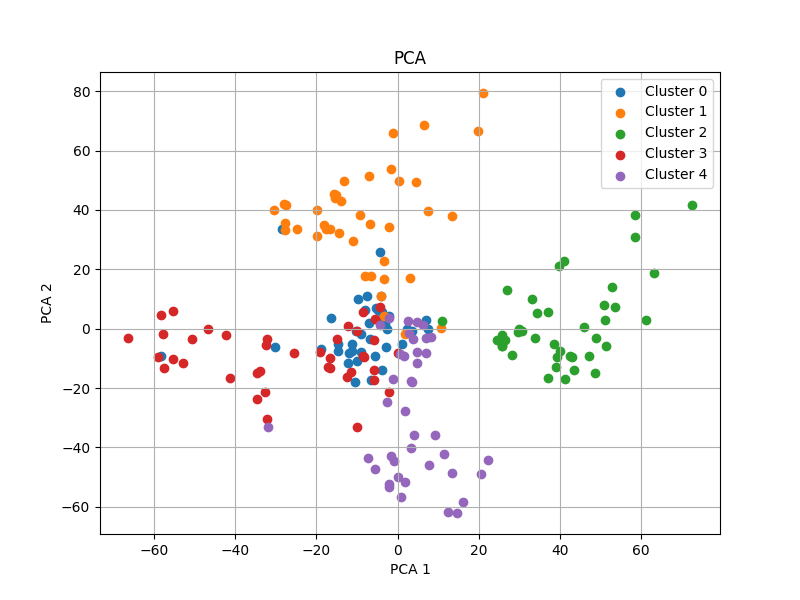
\includegraphics[width=\textwidth]{./Prob4/out/task3_2_mcom2/images/PCA_k5.png}
        \caption{PCA Visualization}
        \label{PCA k5 mcom2 con min20}
    \end{minipage}
    \hfill
    \begin{minipage}{0.32\textwidth}
        \centering
        \includegraphics[width=\textwidth]{./Prob4/out/task3_2_mcom2/images/cluster_result_k5_0_1.png}
        \caption{Age vs. Income}
        \label{fig: Age vs. Annual Income k5 mcom2 con min20}
    \end{minipage}
    \hfill
    \begin{minipage}{0.32\textwidth}
        \centering
        \includegraphics[width=\textwidth]{./Prob4/out/task3_2_mcom2/images/cluster_result_k5_0_2.png}
        \caption{Age vs. Spending}
        \label{fig: Age vs. Spending Score k5 mcom2 con min20}
    \end{minipage}
    \hfill
    \begin{minipage}{0.32\textwidth}
        \centering
        \includegraphics[width=\textwidth]{./Prob4/out/task3_2_mcom2/images/cluster_result_k5_1_2.png}
        \caption{Income vs. Spending}
        \label{fig: Annual Income vs. Spending Score k5 mcom2 con min20}
    \end{minipage}
    \hfill
\end{figure}

\vspace{3em}

\end{document}
